%\documentclass{hitec}
\documentclass{myhitec}
\usepackage[UTF8]{ctex}
\usepackage{fontspec}
\usepackage[dvipsnames]{xcolor}
\usepackage{amsmath}
\usepackage{array}
\usepackage{graphicx}
\usepackage{longtable}
\usepackage{booktabs}  %用于美观表格线宽
\usepackage{multirow}  %用于跨行表
\usepackage{tabularx}  %定义表格宽度
\usepackage{float}
\usepackage{indentfirst}
\usepackage{bibentry}
%\usepackage[linkcolor=gray!40!black]{hyperref}
\usepackage[colorlinks,urlcolor=blue!50!black,linkcolor=blue!50!black,anchorcolor=blue,citecolor=blue!50!black,CJKbookmarks=True]{hyperref}
\usepackage{tcolorbox}
\usepackage{hyperref} % This line is readily ommited of it makes trouble
\tcbuselibrary{breakable,listings,skins,fitting}
\usepackage{newenviron}

%\usepackage{changepage}
%\begin{adjustwidth}{2cm}{1cm}
%\end{adjustwidth}

%==========================================
% Latex 命令环境设置
%==========================================

%==========================================
% 字体设置
%==========================================
%\newfontfamily{\monoca}{Monaco}
\newfontfamily{\monoca}{Microsoft YaHei}
% \setCJKmainfont{FandolSong}
% \setmainfont{FiraSans-Light}
% \setsansfont{FiraSans-Hair}
% \setmonofont{FiraMono-Regular}

\setCJKmainfont{Microsoft YaHei}
% \setmainfont{Microsoft YaHei}
% \setsansfont{Microsoft YaHei}
% \setmonofont{Microsoft YaHei}

\setmainfont{Consolas}
\setsansfont{Consolas}
\setmonofont{Consolas}


%==========================================
% 自定义命令设置
%==========================================
\newcommand{\urllink}[2]{\href{#1}{#2}}

\newcommand{\HT}{\textsc{\raisebox{0.1em}{H}\raisebox{-0.1em}{I}%
	\raisebox{0.1em}{T}\raisebox{-0.1em}{E}\raisebox{0.1em}{C} }}

\newtheorem{thm}{定理}
\newcommand\degree{^\circ}

\newtcbox{\emphasizebox}[1][blue]{enhanced,on line,%drop fuzzy shadow,
arc=2pt,outer arc=2pt,colback=#1!5!white,colframe=#1!50!black,
boxsep=0pt,left=3pt,right=3pt,top=1pt,bottom=1pt,
colupper=blue!50!black,fit basedim=10pt,
boxrule=0.1pt,bottomrule=0.1pt,toprule=0.1pt,nobeforeafter}

%==========================================
% 自定义lsting设置
%==========================================
\newtcblisting{messagebox}{%
breakable,
left=3mm,
listing only,
boxrule=0.2mm,
colback=gray!5,
fontupper=\monoca,colupper=red!50!black,
coltext=black
}%

\newtcblisting{commandbox}{%
breakable,
left=3mm,
listing only,
boxrule=0.2mm,
colback=black,
fontupper=\monoca,colupper=red!50!black,
coltext=green
}%

\newtcblisting{codeout}{%
breakable,
left=3mm,
boxrule=0.2mm,
colback=gray!5,
fontupper=\monoca,colupper=red!50!black,
coltext=black
}%

%\lstset{
    % numbers=left,
    % %numberstyle={\color{lightgray}},
    % numberstyle={\color{green}},
    % backgroundcolor={\color[RGB]{41, 47, 51}}, %背景颜色
    % basicstyle={\color[RGB]{208, 214, 219}}, %普通字符串颜色
    % stringstyle={\color[RGB]{0, 128, 0}}, %字符串颜色
    % keywordstyle={\color[RGB]{101, 140, 230}}, %关键词颜色
    % commentstyle={\color{gray}}, %注释颜色
    % frame=none, %无边框
    % breaklines=true, %自动分行
    % language={[ANSI]C},
    % captionpos=b,
% }

\lstnewenvironment{myccode}[1][]
{\lstset{
    numbers=left,
    %numberstyle={\color{lightgray}},
    %frame=none, %无边框
    frame=lines, %上下线
    %frame=single, %边框
    language={[ANSI]C},
    breaklines=true, %自动分行
    %keywordstyle={\color{blue}}, %关键词颜色
    %stringstyle={\color{orange}}, %字符串颜色
    %stringstyle={\color{magenta}}, %字符串颜色
    %commentstyle={\color{green}}, %注释颜色
    %basicstyle={\color[black]}, %普通字符串颜色
    %captionpos=b,
    #1
        }
}
{}

%==========================================
% 标签格式
%==========================================
\hypersetup{
    colorlinks=true,
    bookmarksnumbered=true,
    pdftitle={My LaTeX2e note},
    pdfkeywords={LaTex, note},
}

%==========================================
% 摘抄格式
%==========================================
\newenvironment{literbox}
%{\begin{messagebox}
{\begin{quote}\zihao{-4}\kaishu
%{\zihao{-3}\kaishu
}
%{\end{messagebox}}
{\end{quote}}
%{}

%==========================================
% 图片路径
%==========================================
\graphicspath{{figure/}, 
{005_protocol_note/bt_picture/}, 
{009_soft_install_note/gvim_install_picture/}, 
{008_system_work_note/system_note_picture/}, 
}

%==========================================
% 水印
%==========================================
%\usepackage{draftwatermark}
%\SetWatermarkText{Zero Note} % the Text
%\SetWatermarkLightness{0.9} % the lightness from 0 to 1, default 0.8
%\SetWatermarkScale{1.0} % the scale, default 1.2


%==========================================
% 首页信息
%==========================================
\title{工作笔记}
\author{莫志烨}
\company{纯属个人}
\confidential{\textbf{-- 非限制发布 --}}

%==========================================
% 开始排版
%==========================================
\begin{document}
\begin{titlepage}
\pdfbookmark[1]{标题页}{title}
\maketitle
这是一篇关于\LaTeX 的文档,风格使用 \HT 。
\end{titlepage}

%\begin{abstract}
%本文说明如何用\LaTeX{}模板撰写报告。
%
%\end{abstract}
%提示:获取本文档的最新版本比现在开始阅读更重要。
%本文的最新版本见于:\url{https://git.coding.net/yangdawei/git.git}
\pdfbookmark[1]{目录}{contents}
\tableofcontents
\newpage
\newpage

%==========================================
% 图片路径
%==========================================
\graphicspath{{figure/},
{002_latex_note/picture/},
{005_protocol_note/bt_picture/},
{005_protocol_note/iis_picture/},
{009_soft_install_note/gvim_install_picture/},
{007_complier_note/picture/},
{008_system_work_note/system_note_picture/},
{010_voa_article/voa_picture/},
}

%==========================================
% 章节内容
%==========================================
\section{\LaTeX 应用笔记}
本文档于\today 开始使用\LaTeX 作笔记文档。

\subsection{超链接应用}
超链接显示有2种:
\begin{itemize}
\item 链接和显示内容一致:\url{https://www.baidu.com}
\item 链接和显示内容不一致:\href{https://www.baidu.com}{百度链接}
\end{itemize}

\subsection{枚举项应用}
以下是枚举内容:
\begin{itemize}
\item 枚举1。
\item 枚举2。
\item 枚举3。
\item 枚举4。
\end{itemize}


\subsection{在正文中强调某个词语}
我要\emphasizebox{强abc调}这个词语。

\subsection{插入Linux命令}
\begin{commandbox}
 > sudo chsh -s zsh
\end{commandbox}

\subsection{用数字表示一个范围}
我要表示一个范围:$18\sim22$ 岁。

\subsection{插入一个Linux信息输出框}
\begin{messagebox}
On branch master
Your branch is ahead of 'origin/master' by 3 commits.
  (use "git push" to publish your local commits)
Changes not staged for commit:
  (use "git add <file>..." to update what will be committed)
  (use "git checkout -- <file>..." to discard changes in working directory)
\end{messagebox}

\subsection{测试codeout}
\begin{codeout}
codeout ccc
\end{codeout}


\subsection{基本代码块测试}
\begin{lstlisting}[language=C, numbers=left]
void main ()
{
    return;
}
\end{lstlisting}

\subsection{测试mycode}
\begin{myccode}
/* 这是一个hello工程 */
void main ()
{
    int cnt = 0;
    printf("Hello World: %d\n", cnt);
    return;
}
\end{myccode}

\subsection{空行分段 单个换行相当于空格}
老话说生活有五味,酸甜苦辣咸。苦是生命所不能避免的一味,叔本华说:“人生就是痛苦,我们可以把痛苦转换成幸福”,努力就是转化的过程,尽管在这个过程中,我们可能会感到更加辛苦。

苦,是人生的必经过程。人生就是一个“享受”痛苦和磨难的过程,这个过程是值得体会和拥有的。
人生本身就是一场与痛苦并存的旅行,并不像很多人想象的那么轻松,从生下来的那一天,我们就开始了人生的修行。

无论你生长在怎样的环
境中,你都会面临人生的各种难题。面对这些难题、困境,没有人可以不流泪流汗就轻轻松松地跨过去。经历得越多,越容易发现这个世界的真理——越怕吃苦,越有苦吃。那些心灵真正富足的人,其实都不怕吃苦。

\subsection{脚注命令}
苦\footnote{\emph 苦,是人生的必经过程。}

\subsection{引用}
\begin{quote}
老话说生活有五味,酸甜苦辣咸。
\end{quote}

\subsection{改变字体和字号}
\begin{quote}
\zihao{-5} \kaishu 老话说生活有五味,酸甜苦辣咸。
\end{quote}

\subsection{定理环境}
\begin{thm}[勾股定理]
一二三。
\end{thm}

\subsection{公式排版}
\begin{equation}
a(b+c) = ab + ac
\end{equation}

\begin{equation}
\angle ABC = \pi / 2
\end{equation}

\begin{equation}\label{eq:gougu}
AB^2 = BC^2 + AC^2
\end{equation}

\begin{equation}
90^\circ
\end{equation}

\subsection{插入图片}
%\begin{figure}[ht]
\begin{figure}[H]
\centering
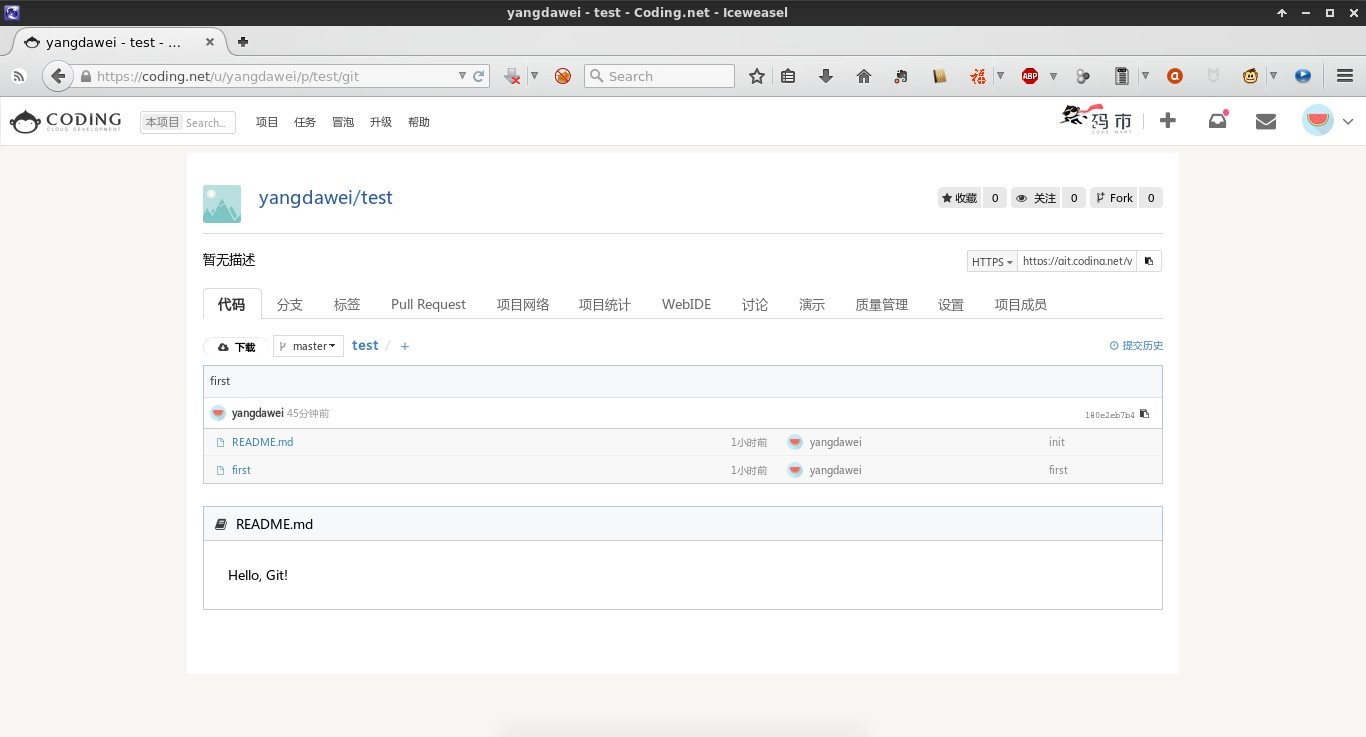
\includegraphics[height=5cm]{testcode.jpg}
\caption{建立项目}
\label{fig:createproject}
\end{figure}

\subsection{插入表格}
\begin{table}[H] %浮动环境
\begin{tabular}{|rrr|}
\hline
直角边 $a$ & 直角边 $b$ & 斜边 $c$ \\
\hline
3 & 4 & 5 \\  %分列
5 & 12 & 13 \\ %下一行
\hline
\end{tabular}
\end{table}

\subsection{引用公式和图表}
图 \ref{fig:createproject} 表示。

公式 \ref{eq:gougu} 方法。

另一种引用公式 \eqref{eq:gougu} 方法。 %添加\usepackage{amsmath}

\subsection{自定义新的命令}
使用newcommand命令。
符号度的新命令 $90\degree$ 。%注意:要加$$

\subsection{一些标点符号}
省略号\ldots \dots \# \quad \$ \quad \% \quad \& \quad \{ \quad \} \quad \_ \quad \textbackslash

中文标点使用全角输入,破折号shift+- ——,省略号shift+6……

忽略每行前面的空格,后面的空格多个当成一个,\TeX\ ing,\TeX{} ing. {\TeX} ing. 换行当空格I 
am Tex.汉字和字母自动添加空格tex。



\section{GIT学习笔记}
\subsection{合并两个提交历史}
连续在本地有两个提交, 如果需要合并这两个提交历史, 使用命令:
\begin{cmd}
 > git rebase -i HEAD~2
\end{cmd}



\section{VIM学习笔记}

\section{通信协议学习笔记}
\subsection{IIC通信协议}

\subsection{UART通信协议}

\subsection{SPI通信协议}

\subsection{IIS通信协议}
\subsubsection{IIS概述}
I2S = Inter-IC Sound = Integrated Interchip Sound = IIS,是飞利浦在1986年定义(1996年修订)的数字音频传输标准,用于数字音频数据在系统内器件之间传输,例如编解码器CODEC、DSP、数字输入/输出接口、ADC、DAC和数字滤波器等。其与IIC无关联。

\subsubsection{IIS硬件结构}
IIS是个相对来说简单的接口协议,没有地址和片选机制。在总线上,只能同时存在一个主设备和发射设备;提供时钟的设备为主设备,可以是发射设备也可以是接收设备,或者是协调两者的其他控制设备。在高端应用场合中,CODEX经常作为主设备以便精确控制IIS的数据流。

%=============================================================%
%                       插入一张图片                          %
%=============================================================%
\begin{figure}[H]
\centering
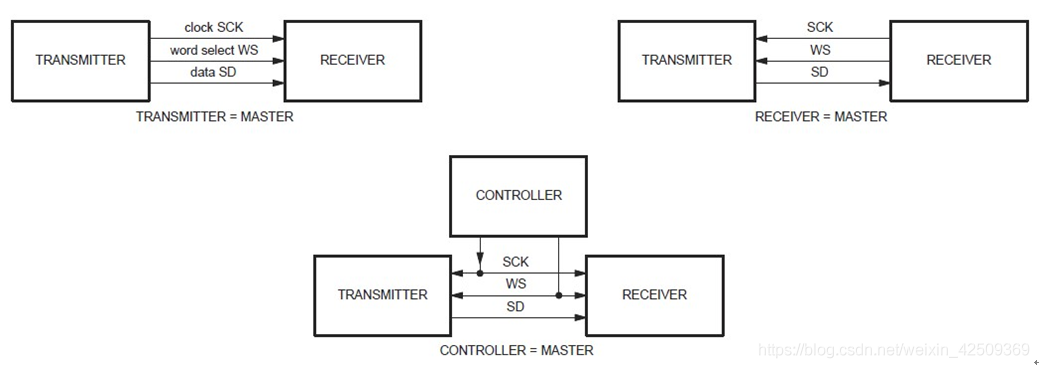
\includegraphics[scale=0.3]{iis_topo.png}
\caption{IIS硬件TOPO结构}
\end{figure}

IIS协议定义三根信号线:时钟信号SCK、数据信号SD和左右声道选择信号WS。
\begin{itemize}
\item WS:声道选择信号,表明数据发送端所选择的声道: WS=0,表示选择左声道,WS=1,表示选择右声道,同时也叫帧时钟,等于声音的采样率。
\item SCK:模块内的同步信号,从模式时由外部提供,主模式时由内部产生。
\item SD:串行数据,以二进制补码形式在数据线上传输;在WS变化后的第一个SCK脉冲,先传输最高位(MSB, Most Significant Bit)。
\end{itemize}

\subsubsection{IIS工作模式}
IIS的操作模式分为三种:标准IIS模式、左对齐模式和右对齐模式。
\begin{itemize}
\item 标准IIS模式(Phillips Standard)

IIS模式是标准左对齐格式再延迟一个时钟位变化来的,时序如下所示:
\begin{figure}[H]
\centering
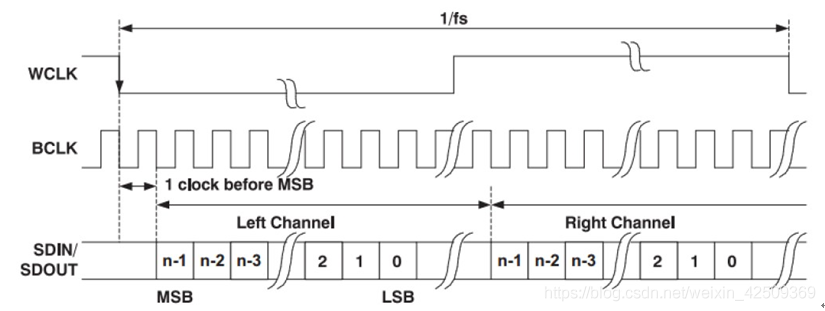
\includegraphics[scale=0.4]{iis_starndar_mode.png}
\caption{标准IIS模式}
\end{figure}
左右通道的数据MSB均是在WS变化后第二个SCK/BCLK上升沿有效。

\item 左对齐模式(Left Justified Standard)

标准左对齐格式的数据的MSB没有相对于BCLK延迟一个时钟。左对齐格式的左右声道数据的MSB在WS边沿变化后SCK/BCLK的第一个上升沿有效。具体如下图所示:
\begin{figure}[H]
\centering
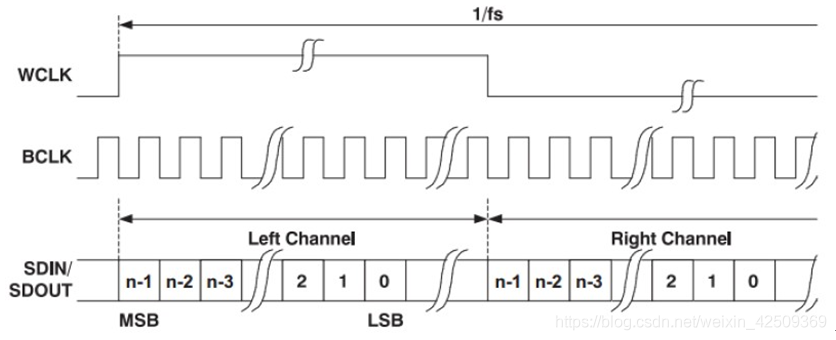
\includegraphics[scale=0.4]{iis_left_mode.png}
\caption{IIS左对齐模式}
\end{figure}
支持16~32bit字长格式;

\item 右边对齐模式(Right Justified Standard)

也叫日本格式,sony格式,具体对齐方式如下图所示:
\begin{figure}[H]
\centering
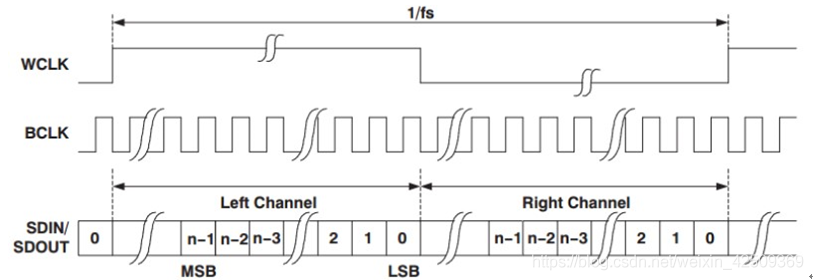
\includegraphics[scale=0.4]{iis_right_mode.png}
\caption{IIS右对齐模式}
\end{figure}
接收设备必须事先知道待传数据的字长。

\end{itemize}

\begin{messagebox}
注意左右对齐模式的WS时钟高电平为左声道,低电平为右声道,刚好与标准IIS相反。
\end{messagebox}

\subsubsection{IIS时钟频率计算}
SCK = 采样率(48K、44.1K、16K等) x  字长(16bit、24bit、32bit) x 2(左右两通道);MCLK/SCK =  384 、256 等需要参考手册说明支持哪种;

\subsubsection{一些问题解答}
\begin{itemize}
    \item \emphasizebox{384, 512fs}代表什么意思?\newline
        256fs中“fs” 就是表示audio sampling frequency, 表示在一个LR周期中BCLK的个数,比如;数据是32bit位宽,2个通道,那么fs就是32 x 2 = 64fs,可以理解为一帧有多少个sclk, fs参数结合采样率(LRCLK)可以算出BCLK,BCLK与MCLK存在分频关系,这个关系与实际通信芯片有关;
\end{itemize}

\subsection{蓝牙通信协议}
\begin{figure}[H]
\centering
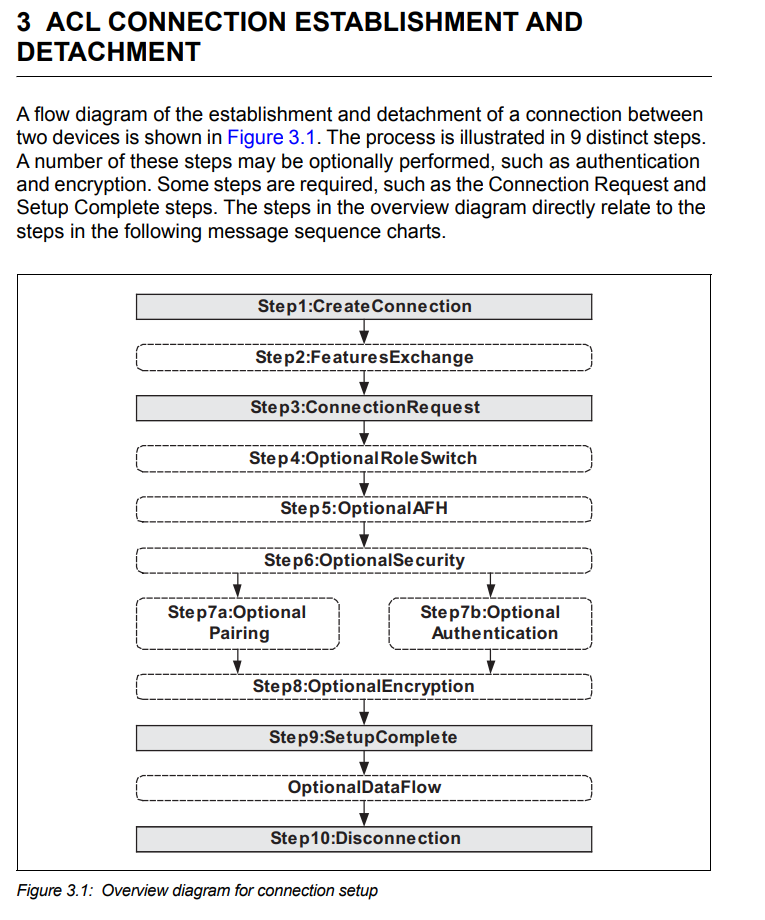
\includegraphics[height=8cm]{connection.png}
\caption{连接步骤}
\label{fig:connection}
\end{figure}

\begin{figure}[H]
\centering
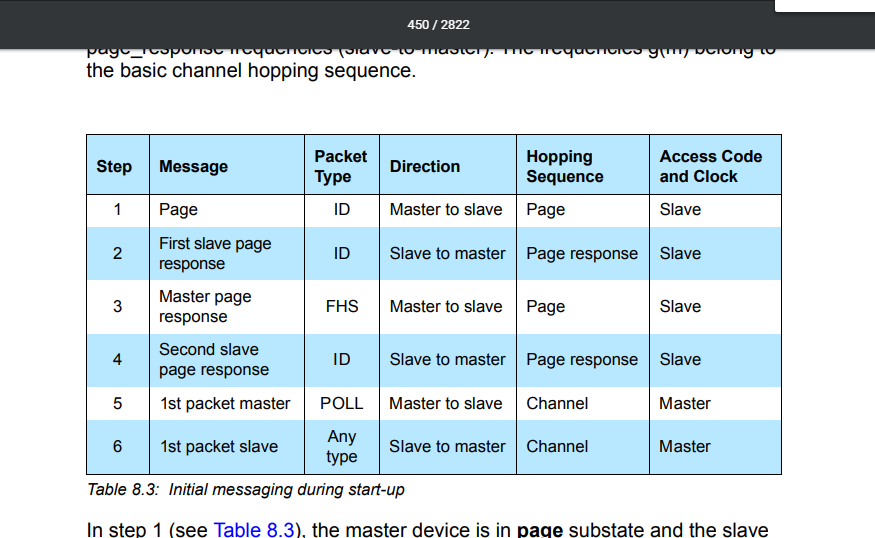
\includegraphics[height=8cm]{page_startup.png}
\caption{pagestartup}
\label{fig:pagestartup}
\end{figure}

\begin{figure}[H]
\centering
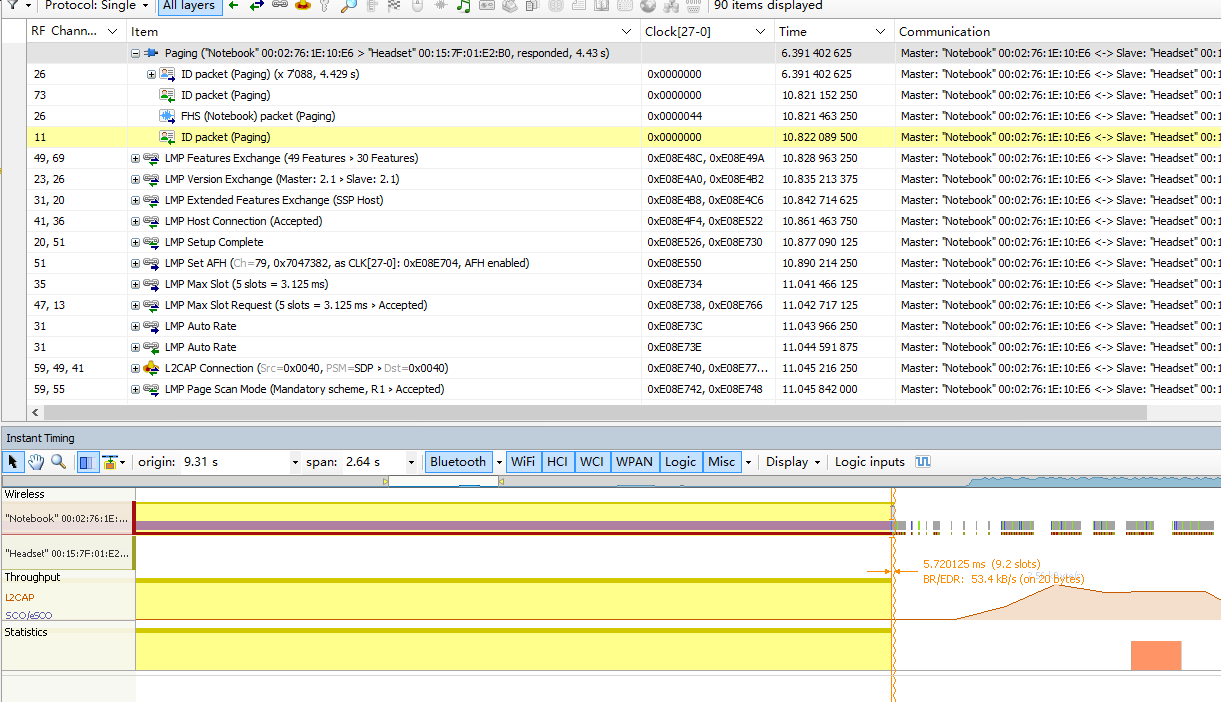
\includegraphics[height=8cm]{page_startup_data.png}
\caption{pagestartupdata}
\label{fig:page_startup_data}
\end{figure}

\href{https://en.wikipedia.org/wiki/Diffie%E2%80%93Hellman_key_exchange}{wiki链接}
\begin{figure}[H]
\centering
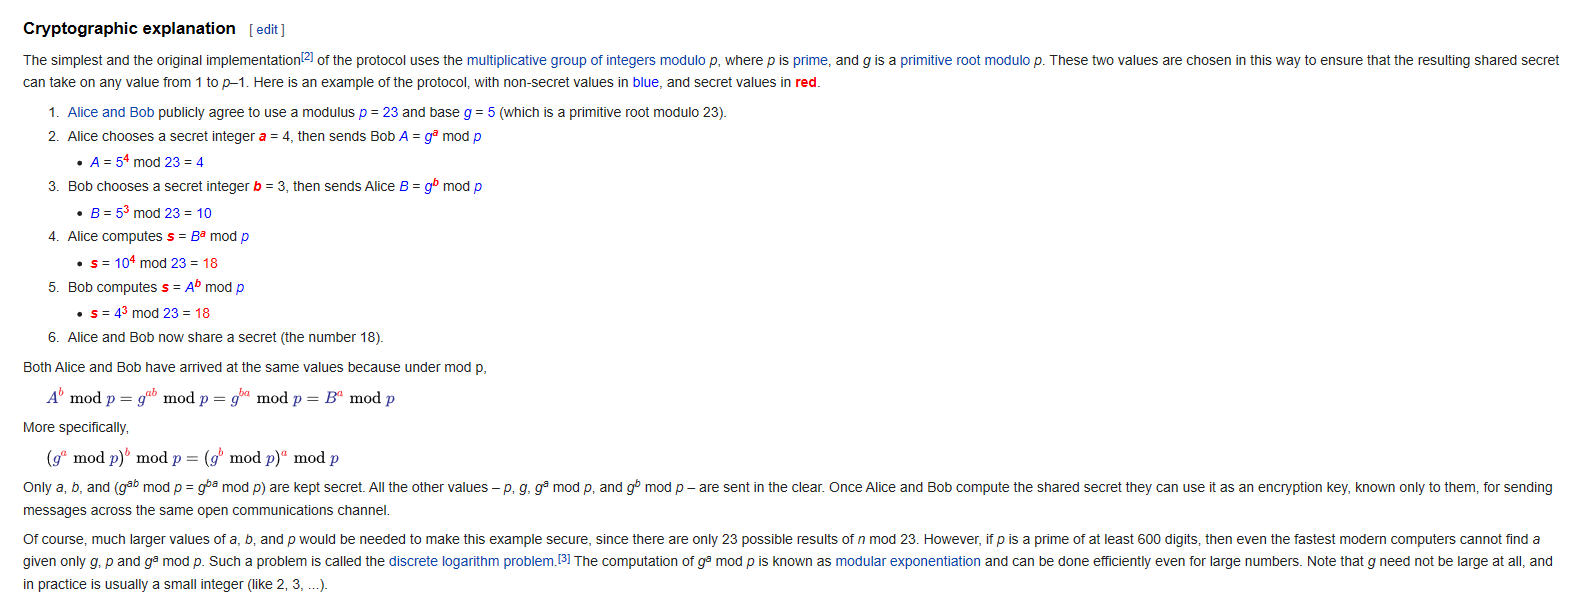
\includegraphics[height=8cm]{wiki1.png}
\caption{wiki1}
\label{fig:wiki1}
\end{figure}

\begin{figure}[H]
\centering
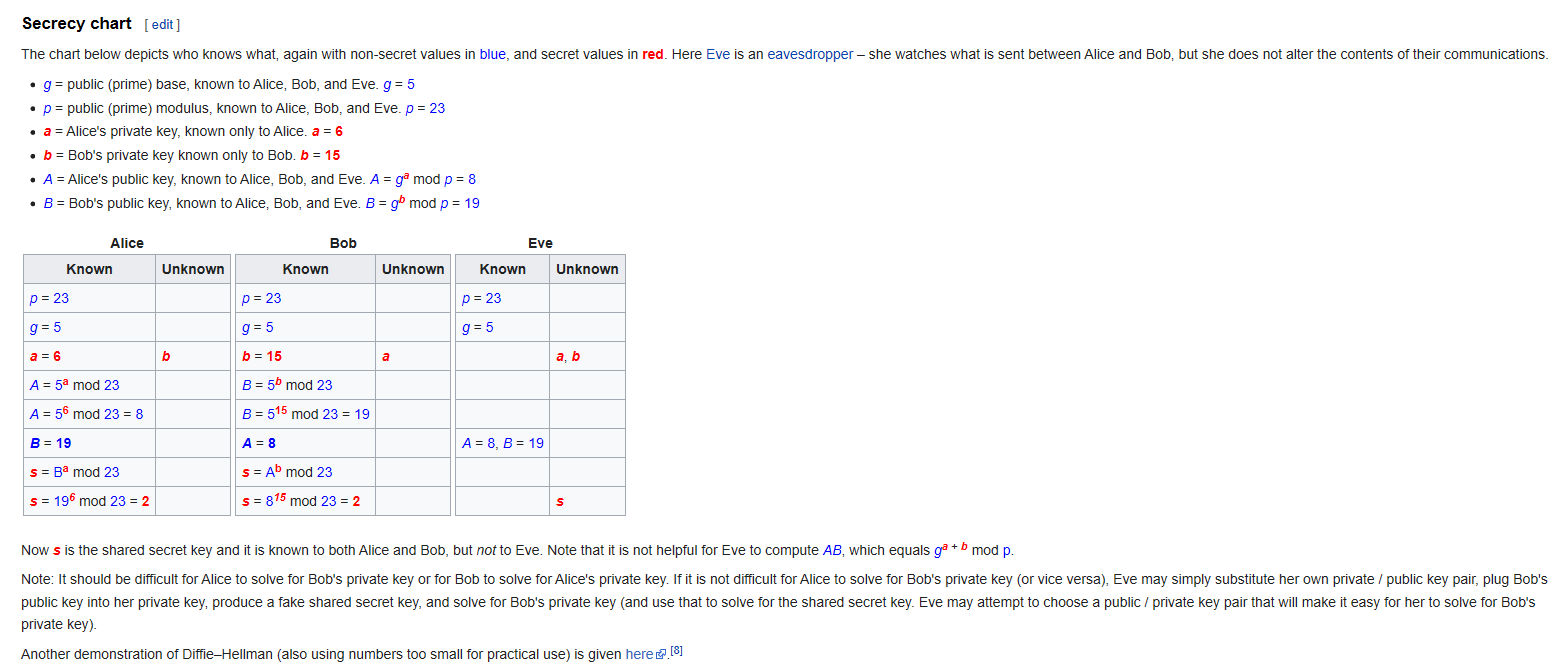
\includegraphics[height=8cm]{wiki2.png}
\caption{wiki2}
\label{fig:wiki2}
\end{figure}

\subsection{USB通信协议}



\section{文学摘抄}
%\begin{itemize}
\subsection{2020年7月28日:《破窑赋》}
%\item 2020年7月28日:《破窑赋》

%\begin{literbox}
    天有不测风云,人有旦夕祸福。蜈蚣百足,行不及蛇;雄鸡两翼,飞不过鸦。马有千里之程,无骑不能自往;人有冲天之志,非运不能自通。

    盖闻:人生在世,富贵不能淫,贫贱不能移。文章盖世,孔子厄于陈邦;武略超群,太公钓于渭水。颜渊命短,殊非凶恶之徒;盗跖年长,岂是善良之辈。尧帝明圣,却生不肖之儿;瞽叟愚顽,反生大孝之子。张良原是布衣,萧何称谓县吏。晏子身无五尺,封作齐国宰相;孔明卧居草庐,能作蜀汉军师。楚霸虽雄,败于乌江自刎;汉王虽弱,竟有万里江山。李广有射虎之威,到老无封;冯唐有乘龙之才,一生不遇。韩信未遇之时,无一日三餐,及至遇行,腰悬三齐玉印,一旦时衰,死于阴人之手。

    有先贫而后富,有老壮而少衰。满腹文章,白发竟然不中;才疏学浅,少年及第登科。深院宫娥,运退反为妓妾;风流妓女,时来配作夫人。

    青春美女,却招愚蠢之夫;俊秀郎君,反配粗丑之妇。蛟龙未遇,潜水于鱼鳖之间;君子失时,拱手于小人之下。衣服虽破,常存仪礼之容;面带忧愁,每抱怀安之量。时遭不遇,只宜安贫守份;心若不欺,必然扬眉吐气。初贫君子,天然骨骼生成;乍富小人,不脱贫寒肌体。

    天不得时,日月无光;地不得时,草木不生;水不得时,风浪不平;人不得时,利运不通。注福注禄,命里已安排定,富贵谁不欲?人若不依根基八字,岂能为卿为相?

    吾昔寓居洛阳,朝求僧餐,暮宿破窑,思衣不可遮其体,思食不可济其饥,上人憎,下人厌,人道我贱,非我不弃也。今居朝堂,官至极品,位置三公,身虽鞠躬于一人之下,而列职于千万人之上,有挞百僚之杖,有斩鄙吝之剑,思衣而有罗锦千箱,思食而有珍馐百味,出则壮士执鞭,入则佳人捧觞,上人宠,下人拥。人道我贵,非我之能也,此乃时也、运也、命也。

    嗟呼!人生在世,富贵不可尽用,贫贱不可自欺,听由天地循环,周而复始焉。
%\end{literbox}

%\end{itemize}

\section{编译器特性笔记}
\subsection{关于versioncheck原理优化代码原理}
Q:编译器代码优化是按照c文件为单位还是以函数为单位,如果以函数为单位,为什么类似于文件系统这些是以version\_check函数调用时,整个c文件的函数都会被调用进来?
\begin{itemize}
\item 函数链接是以\_entry标号作为入口,如果一个函数被显示调用,会把这个函数标号加进来链接,链接是以.o为单位,如果一个函数被显示调用,会把该函数的全部标号拉进来链接(包括结构体),如果一个结构体定义了\emphasizebox{used}属性,该标号会被最终链接进来,导致结构体里的函数指针也会被链接进来,这是使用version\_check选择性链接的原理。

\item libc.a这个库比较特殊,一个函数就是一个.o文件。


\end{itemize}

\subsection{C内联汇编}
参考: \myurlfootnote{https://www.ibiblio.org/gferg/ldp/GCC-Inline-Assembly-HOWTO.html}{GCC-Inline-Assembly-HOWTO}

一般为而言,通过 asm(...) 、 \_\_asm\_\_(...) 、 asm volatile(...) 和 \_\_asm\_\_ volatile(...) 来包含汇编指令模板的字符串形式,如果有额外的约束,通过 : 来分割并指定。
\subsubsection{内联汇编模板}
\begin{myccode}
asm ("汇编模板"
 : /* 输出操作数列表, 可空 */
 : /* 输入操作数列表, 可空 */
 : /* 修改了的寄存器列表, 可空 */
 );

asm ("nop"); // 一条 nop 指令, 没有额外的约束
__asm__ ("nop"); // 同上
 asm volatile ("nop"); // 表示不要随便移动(调度) 这条指令的位置
__asm__ volatile ("nop"); // 同上
\end{myccode}

在一些情况下,在内联汇编中使用了一些指令,这些指令会修改特定的寄存器,这个时候就需要在修改了的寄存器列表里面指明。这是因为内联汇编本身是字符串,并不会被解析,所以编译器内部并不能知道内联汇编的语义(即修改了哪些寄存器、有什么输入输出、做了什么事情以及是否能够被任意移动位置)。所以、我们总是需要通过输出,输入还有修改列表来指定。值得注意的是,为了实现 C 语言的调用协议,一些寄存器被用作了特殊的用途,如使用的栈指针寄存器。

\begin{myccode}
// 下面的做法也是危险的, 因为 r0 被修改了, 但是没有指明
__asm__ volatile ("r0 = 0");
__asm__ volatile ("r0 = 0" : : : "r0"); // ok

//另外一些情况下, 我们可能不希望自己分配寄存器的使用, 可以让编译器分配, 这个是还有需要通过%来指明
u32 reg;
__asm__ volatile ("%0 = rets" : "=r"(reg));
printf("rets的值是 %x", reg);
 // 这个时候表示第0个操作数作为输出, 最终编译器会给%0分配一个寄存器,并替换%0。
\end{myccode}

上述例子中的 "=r"(reg) 表示,对应的内联汇编本体会输出一个结果,并且这个结果应该放置到一个寄存器中,即 "=r" 。而 (reg) 则表示,希望编译器绑定 reg 变量和保存结果的寄存器。这样我们可以而通过访问 reg 获取对应的值。

\subsubsection{多条内联汇编}
一些情况下,会需要写多条连续的内联汇编。这个时候正确的做法是,把这些内联汇编语句用一个 \_\_asm\_\_ 块来表示,而不是分开多个 \_\_asm\_\_ 。例如:
\begin{myccode}
// 定义一个宏, 希望能够清空r1, r0寄存器
// 一个错误的做法:
// 下面的做法有多种错误
// 1. 应该使用一个__asm__块来, 而不是分开多个。 否则它们之间可能会插入其它的指令。
// 2. 内联汇编本体中修改了r1, r0寄存器, 但是没有通过修改列表来说明。
#define MACCLR() __asm__ volatile ("r1 = 0"); __asm__ volatile ("r0 = 0")

// 正确一点的做法:
#define MACCLR() __asm__ volatile( \
"r1 = 0 \n\t" \
"r0 = 0 \n\t" \
: \ // 没有输出
: \ //没有输入
: "r1", "r0" \ // 修改了 r1, r0
);

// 更好一些的做法:
// pi32v2中有一条指令
#define MACCLR() __asm__ volatile ("r1_r0 = 0" : : : "r1", "r0");
\end{myccode}

\subsubsection{寄存器约束}
编译器来分配寄存器的时候,需要指定需要分配的寄存器类型,总结如下:
\begin{figure}[H]
\centering
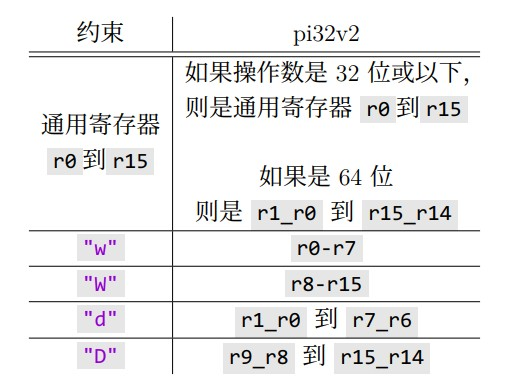
\includegraphics[scale=0.7]{asm_reg.jpg}
\caption{指定分配寄存器}
\label{fig:asm_reg}
\end{figure}
为了方便起见,对于一个 64 位寄存器 DR ,可以用 DR.l 来表示 DR 的低 32 位所在的寄存器, DR.h 用来表示 DR 的高 32 位所在的寄存器。例如r1\_r0.l表示r0,r1\_r0.h表示r1。

\subsubsection{输出约束}
有些时候,我们需要利用内联汇编来获取一些值,这些值需要输出到一些地方,我们通常需要一条输出约束。
\begin{myccode}
unsigned reg;
__asm__ volatile ("%0 = rets" : "=r"(reg));
printf("rets寄存器的值是: %x\n", reg);
// 由上面的汇编说明可以看到, 这个是 pi32v2 的汇编语法
// 表示 %0 表示第一个操作数, 这个是 : 后面开始算起的,
// "=r" 表示这个操作数需要写入到一个寄存器中,
// "=r"(reg) 表示, 输入的寄存器需要和 reg 分配到同一个
// 寄存器, 也就是可以认为把这个结果放入 reg
// 这个指令可以获取当前 rets 的值, 并放入 reg 变量中

__asm__ volatile ("%0 = sp\n" : "=r"(reg));
printf("sp寄存器的值是: %x\n", reg);
// 把 sp 的值存放在 reg 中
__asm__ volatile ("%0 = r4" : "=r"(reg));
printf("r4寄存器的值是 %x\n", reg);
// 获取 r4 的值到 reg 中

__asm__ volatile ("%0 = rets\n" : "=r"(reg));
printf("rets寄存器的值是 %x", reg);
\end{myccode}

\subsubsection{输入约束}
有些时候,我们需要指定一些输入到内联汇编中,这个时候,会需要一条输入约束。
\begin{myccode}
unsigned retaddr = get_retaddr();
__asm__ volatile ("reti = %0\n\t"
"rti \n\t" : : "r"(retaddr));
// "r" 表示这个操作数是被读的, 表示把 retaddr 的值赋值给
// reti, 然后执行 rti 指令, 实现了跳转
\end{myccode}

%值得注意的是,当有多于一条汇编指令需要内联的时候,通常我们写成上述形式,即每行一个汇编指令,并在末尾加上\textbackslash n \textbackslash t,由于内联汇编实际上以字符串形式存储,所以\textbackslash n \textbackslash t 表示换行并插入一个 tab 键。

\subsubsection{earlyclobber 操作数}
编译器在给内联汇编分配寄存器的时候,整块内联汇编被当做一条具有特定输入和输出的指令。并不会关心其内在的含义。例如:
\begin{myccode}
int a, b;
__asm__ volatile (
"%0 = ~ %1\n\t"
: "=r"(a)
: "r"(b));

 //在分配寄存器的过程中, 上面的内联汇编块被当做了
 // <INLINEASM> outs{%0}, ins{%1}
 // 特定于这个例子来说, 如果后续代码不在继续使用 b的值, 而只是使用了a的值
 // 那下面的一些寄存器分配都是合理的
 // 分配方式一:
 // r0 = ~ r0 ; 因为 b 后续不在被使用了, 所以其寄存器可以被a占用
 // 分配方式二:
 // r1 = ~ r0 ; 当然, 也有可能a分配了其它的寄存器
\end{myccode}

另外一些时候,我们的内联汇编块中不会只有一条指令,那么指令之间可能会有先后执行的顺序。这种把所有指令当做一个整体的处理方式,可能会导致问题,例如下面的例子:

\begin{myccode}
int a1, a2;
int b1, b2;
__asm__ volatile (
" %0 = ~ %2\n\t"
" %1 = ~ %3\n\t"
: "=r"(a1), "=r"(a2)
: "r"(b1), "r"(b2)
 );

 // 假设 b2, b1都不在这条指令之后被使用
 // 同样的, 这里在分配寄存器的时候, 还是会被当做下面的东⻄
 // <INLINEASM> outs{%0, %1}, ins{%2, %3}
 // 显然, 如果这个内联块能够作为一条指令整体执行完,
 // 那么下面的一些寄存器分配都是合理的
 // 分配方式一:
 // <INLINEASM> outs{r0, r1}, ins{r0, r1}
 // 即
 // r0 = ~ r0
 // r1 = ~ r1
 // 分配方式二:
 // <INLINEASM> outs{r1, r0}, ins{r0, r1}
 // 即
 // r1 = ~ r0
 // r0 = ~ r1
 // 但是这里, 第二种方式会导致错误的代码
\end{myccode}

上面的例子中,第二种分配方式,如果从一条指令的情况来看,是合理的。毕竟所有的输入一次性使用完毕,然后同时所有的输出被赋值完毕。但是问题在于,输入并不是一次性使用完毕,输出也不是一次性赋值完毕。而是使用一些输入(这里来说,就是第一条 not 指令),然后定义了一些输出,然后又使用了一些输入(这里来说,就是第二条 not 指令),再定义了一些输出。所以,我们需要一个方式标记一些输出,告知编译器这些输出被赋值的时候,还有一些输入没有被使用完,所以,不要让这些输出所使用的寄存器占用输入所使用的寄存器。这种标记方式就是\& 。上面的例子需要修正为

\begin{myccode}
int a1, a2;
int b1, b2;
__asm__ volatile (
" %0 = ~ %2\n\t"
" %1 = ~ %3\n\t"
: "=&r"(a1), "=r"(a2)
: "r"(b1), "r"(b2)
);
// 假设 b2, b1都不再这条指令之后被使用
// & 表示 a1 定义的时候, 输入还没有使用完毕, 也就是说
// 不应该把 a1 定义到 b2, b1 占用的寄存器上
// 对于 a2, 因为 a2 已经是最后一个定义的寄存器, 可以不用加上&
// 因为定义a2的时候, 所有的输入已经使用完毕了
// 当然, 加上也是可以的
\end{myccode}

\subsubsection{输入的同时是输出}
有些操作数是既有读属性,又有写属性的:比如一个后加指令的基地址寄存器,在访问内存后,基地址寄存器的值会被更新,对于这些指令,我们需要两条约束来指定。
\begin{myccode}
void t2sos16(short *in, short *out, int *coeff, int *mem, int npoint, intdstep) 
{
    const int coeffQ = 20;
    const int LeftBit = 8;
    int tmp32_1, tmp32_2, tmp32_3;
    long long tmp64_1;
    asm volatile (
    " %0 += 2<<2 \n\t"
    " %7 = %7 << 1 \n\t"
    "1: \n\t"
    " \n\t"
    " %1 = h[%8++=0] * [%0++=1<<2] (s) \n\t"
    " %4 = %1 >> (%20-%21) (s) # %5 = [%3+0] \n\t"
    " %5 += %4 \n\t"
    " %1 = [%0++=-3<<2] * %4 (s) \n\t"
    " %1 += [%0++=4<<2] * %5 (s) \n\t"
    " %1.l = %1 >>> %20 (up) # %6 = [%3+1<<2] \n\t"
    " %6 += %1.l \n\t"
    " %1 = [%0++=-3<<2] * %4 (s) \n\t"
    " %1 += [%0++=1<<2] * %5 (s) \n\t"
    " %1.l = %1 >>> %20 (up) # [%3+0] = %6 \n\t"
    " %8 += %7 # [%3+1<<2] = %1.l \n\t"
    " %5 >>>= %21 \n\t"
    " %5 = sat16(%5) (s) \n\t"
    " h[%9++=%7] = %5 \n\t"
    " \n\t"
    "if (--%2!=0) goto 1b \n\t"
     : "=&r"(coeff), // 第 0 个操作数, 对应于模板中的 %0
    "=&d"(tmp64_1), // 第 1 个操作数, 对应于模板中的 %1
    "=&w"(npoint), // 第 2 个操作数, 对应于模板中的 %2
    // w 约束了寄存器分配范围, 这是指令要求
    "=&w"(mem), // 第 3 个操作数, 对应于模板中的 %3
    "=&w"(tmp32_1), // 第 4 个操作数, 对应于模板中的 %4
    "=&w"(tmp32_2), // 第 5 个操作数, 对应于模板中的 %5
    "=&w"(tmp32_3), // 第 6 个操作数, 对应于模板中的 %6
    "=&r"(dstep), // 第 7 个操作数, 对应于模板中的 %7
    "=&r"(in), // 第 8 个操作数, 对应于模板中的 %8
    "=&r"(out) // 第 9 个操作数, 对应于模板中的 %9
    : "0"(coeff), // 表示这个操作数需要和 %0 操作数分配到同一个寄存器
    // 这是因为 %0 用作了后加访存指令的基地址操作数, 所以
    // %0 既是一个输入, 也是一个输出
    // "=r"(coeff) 说明了输出, "0"(coeff) 说明同时也是一个输入
    "1"(tmp64_1),
    "2"(npoint),
    "3"(mem),
    "4"(tmp32_1),
    "5"(tmp32_2),
    "6"(tmp32_3),
    "7"(dstep),
    "8"(in),
    "9"(out),
    "i"(coeffQ), // i 表示一个立即数
    "i"(LeftBit)
    :);
}
\end{myccode}

这个例子里面的 coeff 、 tmp64\_1 等,都是既需要读也许要写的操作数。 "=\&r" 表示对应的操作数在指令的输入寄存器使用完成之前就被修改了,这样编译器就不会把输入列表用到的寄存器分配给这些寄存器,这样标记不会导致一些寄存器分配的问题。值得注意的是, "0"(coeff) 之类的约束应该要放置到后面,以防影响操作数顺序。如下面的例子:
\begin{myccode}
int insert(int val_dst, int val_src, int pos, int len)
{
    int pat = (pos << 5) | len;
    __asm__ volatile (
    "%0 <= insert(%1, %2[12:8], %2[4:0])"
    : "=&r"(val_dst),
    : "r"(val_src),
    "r"(pat),
    "0"(val_dst) // 写在最后, 以防影响 %0, %1, %2 顺序
    );

    return val_dst;
}
\end{myccode}

\subsubsection{访问内存}
有时候,我们在内联汇编里面修改了内存,但是由于编译器不知道这个事实,将会导致一些问题。为了解决这个问题,我们需要 "memory" 约束。
\begin{myccode}
// "memory"
int *p = get_ptr();
put_u32hex(*p);
int np = *p + 1;
__asm__ volatile ("[%1] = %0"
: // 没有输出列表
: "r"(np), // 第零个操作数, 对应 %0
// 把 np 的值写入到 *p 的位置
"r"(p) // 第一个操作数, 对应 %1
 : "memory" // 表示内存被修改了
 );
 put_u32hex(*p); // 如果没有上面的 "memory" 可能这个的输出和上一个一样
\end{myccode}

当内联汇编修改了内存的时候,最好加上 "memory" ,这样编译器会失效掉一些缓存了的内存的值。例如上面的 *p ,不过不指定 "memory" 则编译器可能会缓存这个值(为了减少内存访问操作)。

一些例子:
\begin{myccode}
int add(int a, int b)
{
    int c;
    __asm__ volatile (
    "%0 = %1 + %2"
    : "=r"(c) // %0
    : "r"(a), // %1
    "r"(b)); // %2

     // 即 c = a + b
     return c;
}

int add_mem(int *pa, int *pb)
{
    int a, b;
    __asm__ volatile (
    "%0 = [%2] \n\t"
    "%1 = [%3] \n\t"
    "%0 = %0 + %1 \n\t"

    :
    "=&"(a), // %0 输出, 且不能和输入同一个寄存器(⻅earlyclobber操作数)
    "=r"(b) // %1 输出, 可以和输入同一个寄存器
    // (因为定义 %1 的时候, 所有输入都已经使用完毕)
    : "r"(pa), // %2 只是输入
    "r"(pb) // %3 只是输入
);

// 实现了 return *pa + *pb;
return a;
}
\end{myccode}

\section{系统问题总结}
\subsection{关于系统软关机复位问题}
Q:系统软关机使用内置触摸和普通IO关机,开机时\emphasizebox{reset}位置有什么不同?
\begin{itemize}
    \item 普通IO关机,P11系统会掉电,指剩下P33维持电压,开机\emphasizebox{reset}是从\emphasizebox{maskrom}的\emphasizebox{startup}开始;
    \item 使用内置触摸关机,P11系统维持电源工作,这是关机之后还会大几\emphasizebox{uA}的原因,开机\emphasizebox{reset}也是从\emphasizebox{maskrom}的\emphasizebox{Startup}开始;
\end{itemize}

\subsection{关于使用内置触摸开机ROM中IO状态恢复出错问题}
Q:当使用内置触摸开机时,发现\emphasizebox{PC3 IO}变为输出低状态,关机之前在mask\_IO中已经把IO状态设置为高阻?
\begin{itemize}
    \item 当使用\emphasizebox{LPCTMU}关机时,会使用\emphasizebox{PLCNT}模块,配置了\emphasizebox{P3\_PCNT\_SET0}和\emphasizebox{P3\_PCNT\_SET1}两个寄存器,\emphasizebox{PC3 IO}状态正好配置了3,导致在mask恢复IO时设置为输出0状态;
    \item 解决办法:在\emphasizebox{soft\_off\_enter}和\emphasizebox{soft\_off\_exit}时加入\emphasizebox{save}和\emphasizebox{recover}流程即可。
\end{itemize}

\subsection{br28 ass ASS\_CLK\_CON bit7写完和读出来不一样问题(bit5)}
问题:在写ASS\_CLK\_CON的bit7置1时,写完读出来是0x40,再写bit7置0时,读出来时0x20;

解释:由于bit5没有用到,cpu读会移位,在软件层面第一次写bit7置1时,cpu行为:
\begin{myccode}[caption={bit7置1 cpu行为}]
    {
        int bak = 0;
        bak = ASS_CLK_CON;
        bak |= BIT(7);
        ASS_CLK_CON = bak;
    }
\end{myccode}
由于bit5没用到,在cpu读时,bit6变bit5,bit7变bit6,因此写完bit7之后,读出来是0b0100,0000 = 0x40,再把bit7写0时,cpu行为:
\begin{myccode}[caption={bit7置0 cpu行为}]
    {
        int bak = 0;
        bak = ASS_CLK_CON;  //此时bak = 0b0100,0000
        bak &= ~BIT(7);     //此时bak = 0b0100,0000
        ASS_CLK_CON = bak;  //写bit7为0无效;
    }
\end{myccode}
下次再写bit7,将会读回来是0b1100, 0000 = 0xC0,导致出错,硬件Bug;

\subsection{br34 RVDD电压要大于等于DVDD问题}
如果RVDD < DVDD时,有的板子会出现程序跑到某个ram地址出现非对齐访问异常问题。
\begin{figure}[H]
\centering
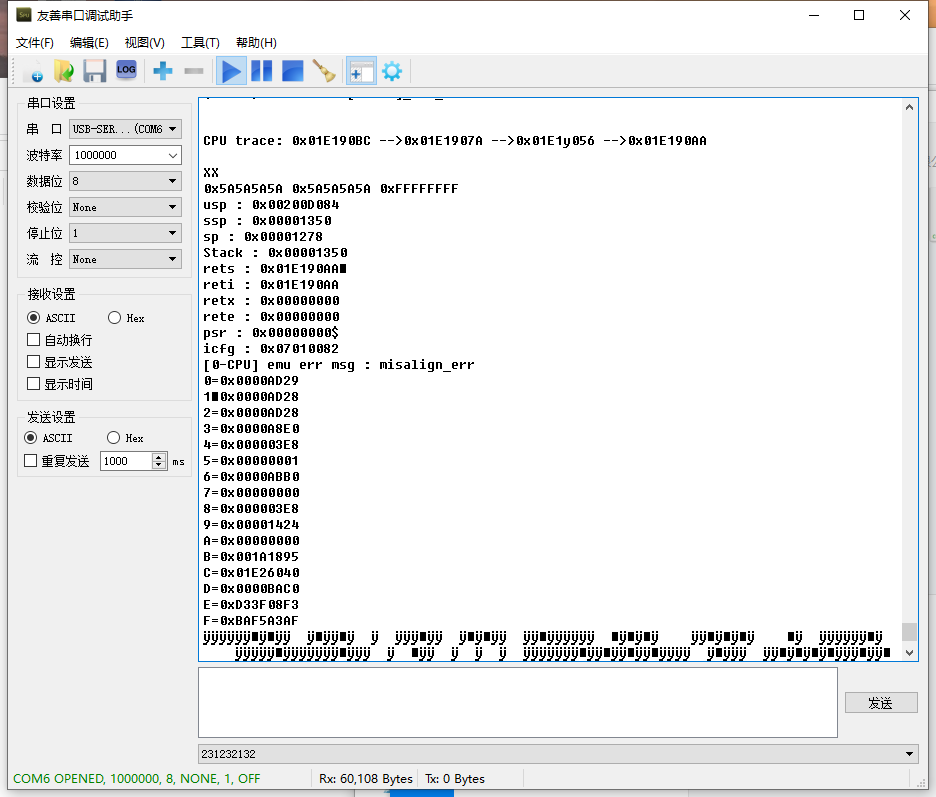
\includegraphics[height=8cm]{rvdd_question.png}
\caption{异常打印}
\label{fig:rvdd_exeception}
\end{figure}
注意:RVDD >= DVDD。


\subsection{有符号数十六进制转十进制计算方法}
计算机内存数值存储方式
1)原码:一个数的原码(原始的二进制码)有如下特点:
\begin{itemize}
\item 最高位做为符号位,0表示正,1表示负
\item 其它数值部分就是数值本身绝对值的二进制数
\item 负数的原码是在其绝对值的基础上,最高位变为1
\item 原码表示法简单易懂,与带符号数本身转换方便,只要符号还原即可,但当两个正数相减或不同符号数相加时,必须比较两个数哪个绝对值大,才能决定谁减谁,才能确定结果是正还是负,所以原码不便于加减运算
\end{itemize}

2)反码
\begin{itemize}
\item 对于正数,反码与原码相同
\item 对于负数,符号位不变,其它部分取反(1变0,0变1)
\item 反码运算也不方便,通常用来作为求补码的中间过渡
\end{itemize}

3)补码
\begin{itemize}
\item 对于正数,原码、反码、补码相同
\item 对于负数,其补码为它的反码加1
\item 补码符号位不动,其它位求反,最后整个数加1,得到原码
\item 在计算机系统中,数值一律用补码来存储
\end{itemize}

4)计算机系统中,数值一律用补码来存储,主要原因是:
\begin{itemize}
\item 统一了零的编码,0在计算机中存储的方式:
\begin{myccode}[caption=zero 编码]
        int a = 0; int b = -0;
        0000 0000     1000 0000
\end{myccode}
\item 为了统一0的编码,计算机中没有-0的概念
\item 将符号位和其它位统一处理,在数据计算中,符号位也参与程序的计算
\item 将减法运算转变为加法运算,计算机只会算加法10+(-10)
\item 两个用补码表示的数相加时,如果最高位(符号位)有进位,则进位被舍弃
\end{itemize}

5)将一个十六进制的有符号数转换为十进制数实例:
\begin{itemize}
\item 十六进制数:0xFFF4 = 0b1111,1111,1111,0100
\item 除了符号位求反码: = 0b1000,0000,0000,1011
\item 原码 = 反码+1:    = 0b1000,0000,0000,1100
\item 原码十进制 = -12
\end{itemize}


\section{软件安装总结}
\subsection{GVIM安装}
\begin{itemize}
\item GVIM安装包链接:\url{https://pan.baidu.com/s/1PcF6-taEaOIg66kbnm6EPA},提取码:66u3。
\item 解压压缩包到任意目录。
\item 运行\emphasizebox{install.exe}
\begin{messagebox}
This program sets up the installation of Vim 8.1

Inspecting system...


Install will do for you:
 1  Install .bat files to use Vim at the command line:
 2      Create C:\WINDOWS\vim.bat
 3      Create C:\WINDOWS\gvim.bat
 4      Create C:\WINDOWS\evim.bat
 5      Create C:\WINDOWS\view.bat
 6      Create C:\WINDOWS\gview.bat
 7      Create C:\WINDOWS\vimdiff.bat
 8      Create C:\WINDOWS\gvimdiff.bat
 9      Create C:\WINDOWS\vimtutor.bat
10  Do NOT change startup file D:\Vim_8_1\_vimrc
14  Install an entry for Vim in the popup menu for the right
    mouse button so that you can edit any file with Vim
15  Add Vim to the "Open With..." list in the popup menu for the right
    mouse button so that you can edit any file with Vim
16  Add Vim to the Start menu
17  Create a desktop icon for gVim
18  Create a desktop icon for gVim Easy
19  Create a desktop icon for gVim Read-only
20  Do NOT create plugin directories
To change an item, enter its number

Enter item number, h (help), d (do it) or q (quit):
\end{messagebox}
\item 选项14是在文件夹空白地方右击弹出vim,不需要点文件;
\item 选项15是在文件夹里的文件右击弹出vim;
\item 实际选择15即可;
\item 注意输入方法, 先输入15,回车\emphasizebox{Enter}
\item 再输入d(do), 回车\emphasizebox{Enter}
\item 添加全局变量,在系统变量添加路径;
\begin{messagebox}
D:\Vim_8_1\vimfiles\tools
\end{messagebox}
\item 直接右击文件用vim打开即可,但还存在字体兼容问题;
\item 安装字体,文件路径
\begin{messagebox}
D:\Vim_8_1\vimfiles\fonts\airline\UbuntuMono
\end{messagebox}
\item 可使用\emphasizebox{RightMenuMgr}工具增加右击打开\emphasizebox{GVIM}
\end{itemize}

\section{VOA文章}
\subsection{2020年8月25日}
\paragraph{\href{https://www.51voa.com/VOA\_Special\_English/covid--plasma-a-breakthrough-or-an-experiment-85234.html}{原文}}
By Hai Do
24 August 2020
Convalescent plasma, which has long been used to treat diseases, has become the latest issue in the race to find treatment for COVID-19.
On Sunday, President Donald Trump announced that the United States would permit the emergency use of convalescent plasma to treat COVID-19 patients. Trump called it "a breakthrough."
However, the World Health Organization (WHO) on Monday warned that the treatment is still experimental. The group described the evidence in support of the treatment as "low quality."
Trump made the plasma announcement after his administration accused the U.S. Food and Drug Administration (FDA) of delaying in order to hurt his re-election chances this November.
The emergency approval makes it easier for some patients to get the treatment. However, it is not the same as full FDA approval for treatment.
\begin{figure}[H]
\centering
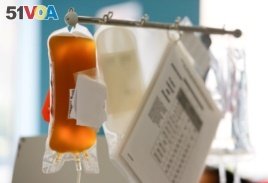
\includegraphics[scale=0.7]{001_voa_20200825.jpg}
\caption{ILE - Convalescent plasma from a recovered coronavirus disease patient.}
\end{figure}
In its announcement, the FDA said, "it is reasonable to believe that COVID-19 convalescent plasma may be effective in lessening the severity or shortening the length of COVID-19 illness in some hospitalized patients." The agency said that more human trials are needed, "as COVID-19 convalescent plasma does not yet represent a new standard of care based on the current available evidence."
Soumya Swaminathan is Chief Scientist at the WHO. She said only a few human trials of convalescent plasma have produced results. "At the moment, it's still very low-quality evidence," Swaminathan told reporters Monday.
The WHO said one Chinese study showed plasma from people who have recovered from coronavirus failed to make a difference in hospitalized patients, while another showed it can lower the risk of death.
What is convalescent plasma?
The treatment involves giving plasma from recovered COVID-19 patients to sick ones. Plasma is the liquid part of blood. Plasma from recovered patients is filled with antibodies, proteins that can kill harmful viruses and bacteria.
The treatment was used during the 1918 flu pandemic. It was also used to fight several other infections before modern medicine found new anti-viral drugs.
Earlier this month, researchers at the Mayo Clinic, in Minnesota, reported data from its experimental program to treat COVID-19 patients around the U.S. with convalescent plasma.
The program called "Expanded Access Program" was not an official study. It did not provide enough information to guarantee that the treatment cured COVID-19. It was "designed to increase access to investigational convalescent plasma and evaluate the safety of this experimental therapy."
The health organization said 70,00 patients received the treatment. It found fewer deaths among those who received the plasma within three days of COVID-19 diagnosis.
Dr. Michael Joyner is lead researcher for the program. He said, "Our hope is that the safety findings and possible efficacy signals could inform the body of knowledge about the use of convalescent plasma to modify the course of COVID-19."
I'm Caty Weaver.
Hai Do wrote this story for Learning English with additional reporting from Reuters and the Associated Press. Caty Weaver was the editor.

\begin{messagebox}
Words in This Story
convalescent - adj. recovering from an illness
plasma - n. the watery part of blood that contains blood cells
illness - n. a condition of being unhealthy, sick
standard - n. a level quality or achievement that is considered acceptable
pandemic - n. an occurrence in which a disease spreads very quickly and affects a large number of people around the world
access - n. a way of getting something
evaluate - v. to judge the value or condition carefully
\end{messagebox}

\paragraph{\href{https://www.51voa.com/VOA\_Special\_English/covid--plasma-a-breakthrough-or-an-experiment-85234_1.html}{翻译}}

Convalescent plasma, which has long been used to treat diseases, has become the latest issue in the race to find treatment for COVID-19.
长期以来一直被用于治疗疾病的康复者血清已经成为了寻找新冠肺炎疗法竞赛中的最新话题。
On Sunday, President Donald Trump announced that the United States would permit the emergency use of convalescent plasma to treat COVID-19 patients. Trump called it "a breakthrough."
川普总统周日宣布,美国将批准康复者血清用于治疗新冠肺炎患者的紧急使用。川普称其为“一次突破。”

However, the World Health Organization (WHO) on Monday warned that the treatment is still experimental. The group described the evidence in support of the treatment as "low quality."
然而,世卫组织周一警告说,这种疗法仍然处于试验阶段。该组织称这种疗法的支持证据“质量不高。”

Trump made the plasma announcement after his administration accused the U.S. Food and Drug Administration (FDA) of delaying in order to hurt his re-election chances this November.
在川普政府指责美国食品药品监督管理局故意拖延以损害他今年11月的连任机会之后,川普发布了这篇血清通告。

The emergency approval makes it easier for some patients to get the treatment. However, it is not the same as full FDA approval for treatment.
这次紧急批准使得一些患者更容易接受到这种治疗。然而,这与美国食品药品监督管理局完全批准这种疗法有所区别。

In its announcement, the FDA said, "it is reasonable to believe that COVID-19 convalescent plasma may be effective in lessening the severity or shortening the length of COVID-19 illness in some hospitalized patients." The agency said that more human trials are needed, "as COVID-19 convalescent plasma does not yet represent a new standard of care based on the current available evidence."
美国食品药品监督管理局在声明中表示,“有理由相信,新冠肺炎康复者血清可以有效减轻某些住院患者的病情或缩短其病程。”该机构表示,还需要进行更多人体试验,“因为根据现有证据,新冠肺炎康复者血清尚不能代表一种新的治疗标准。”

Soumya Swaminathan is Chief Scientist at the WHO. She said only a few human trials of convalescent plasma have produced results. "At the moment, it's still very low-quality evidence," Swaminathan told reporters Monday.
苏米亚·斯瓦米纳坦是世卫组织的首席科学家。她表示,只有少数几项关于康复者血清的人体试验产生了效果。斯瓦米纳坦周一对记者表示:“目前,这仍然算非常低质量的证据。”

The WHO said one Chinese study showed plasma from people who have recovered from coronavirus failed to make a difference in hospitalized patients, while another showed it can lower the risk of death.
世卫组织表示,中国的一项研究表明,来自新冠病毒康复者的血清未能让住院患者产生差异,而另一项研究表明,它可以降低死亡风险。

What is convalescent plasma?
什么是康复者血清?

The treatment involves giving plasma from recovered COVID-19 patients to sick ones. Plasma is the liquid part of blood. Plasma from recovered patients is filled with antibodies, proteins that can kill harmful viruses and bacteria.
这种疗法将新冠肺炎康复者的血清注射给患病患者。血清是血液的液体部分。康复者血清中充满了可以杀死有害病毒和细菌的抗体和蛋白质。

The treatment was used during the 1918 flu pandemic. It was also used to fight several other infections before modern medicine found new anti-viral drugs.
这种疗法在1918年的大流感期间被使用过。在现代医学发现新的抗病毒药物之前,它还被用于抵抗另外几种感染。

Earlier this month, researchers at the Mayo Clinic, in Minnesota, reported data from its experimental program to treat COVID-19 patients around the U.S. with convalescent plasma.
本月初,明尼苏达州梅奥诊所的研究人员报告了一项实验项目中的数据,该项目利用康复者血清治疗美国各地的新冠肺炎患者。

The program called "Expanded Access Program" was not an official study. It did not provide enough information to guarantee that the treatment cured COVID-19. It was "designed to increase access to investigational convalescent plasma and evaluate the safety of this experimental therapy."
这项被称为“Expanded Access Program”的项目并非官方性质的研究。它没有提供足够信息来保证这种疗法可以治愈新冠肺炎。它的目的是“推动康复者血清的调查并评估这种试验疗法的安全性。”

The health organization said 70,00 patients received the treatment. It found fewer deaths among those who received the plasma within three days of COVID-19 diagnosis.
这家卫生机构表示,有7千名患者接受了这种治疗。该机构发现,在新冠肺炎确诊3天内接受这种血清治疗的患者的死亡率更低。

Dr. Michael Joyner is lead researcher for the program. He said, "Our hope is that the safety findings and possible efficacy signals could inform the body of knowledge about the use of convalescent plasma to modify the course of COVID-19."
迈克尔·乔伊纳博士是该项目的首席研究员。他说:“我们希望这种安全结论和可能疗效信号可以提供关于使用康复者血清改变新冠肺炎病程的主体知识。”
\paragraph{\href{https://files.21voa.com/202008/covid-19-plasma-a-breakthrough-or-an-experiment.mp3}{音频}}


\subsection{2021年1月4日}
\paragraph{\href{https://www.51voa.com/VOA\_Special\_English/scientists-declare-climate-emergency-83245.html}{原文}}

\begin{figure}[H]
\centering
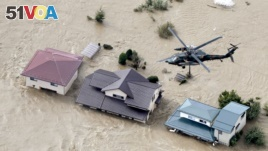
\includegraphics[scale=0.7]{002_voa_20210104.jpg}
\caption{An aerial view shows a Japan Self-Defence Force helicopter flying over residential areas flooded by the Chikuma river following Typhoon Hagibis in Nagano, central Japan, October 13, 2019, in this photo taken by Kyodo.}
\end{figure}

%\begin{messagebox}
By Jonathan Evans
09 November, 2019
More than 11,000 scientists are warning that the Earth, in their words, "clearly and unequivocally faces a climate emergency."
The scientists represent several fields of study and come from 150 countries around the world. They approved a report that appeared in the publication Bioscience earlier this month. It warns that the world would face "untold human suffering" if it does not make deep and lasting shifts in human activities that influence climate change.
The new report is called the "World Scientists' Warning of a Climate Emergency." Three leaders of the study are from the United States. They are ecologists Bill Ripple and Christopher Wolf of Oregon State University and William Moomaw of Tufts University in Massachusetts. The three worked on the study with scientists from universities in South Africa and Australia.
This is the first time a large group of scientists have jointly used the word "emergency" when talking about climate change.
"Despite 40 years of global climate negotiations...we have generally conducted business as usual and have largely failed to address this predicament," the study said. "Climate change has arrived and is accelerating faster than many scientists expected."
The report identified six areas that the world needs to deal with immediately. The scientists appealed to nations to use energy more efficiently and cut their use of fossil fuels. They suggested that lawmakers approve taxes on the burning of carbon-based fuels, such as coal, oil and natural gas.
The scientists expressed support for women's rights and making family planning services "available to all people." They said this would help to reduce sudden or unexpected changes in the size of the human population.
The report urges people to move toward more of a plant-based diet.
Other areas of concern include preventing the destruction of forests and permanent loss of some plant and animal species.
The reported noted that it will most likely take strong actions by the public to move politicians to approve lasting policy changes.
The scientists added, "We believe that the prospects will be greatest if decision-makers and all of humanity promptly respond to this warning and declaration of a climate emergency, and act to sustain life on planet Earth, our only home."
I'm Jonathan Evans.
VOANews.com reported this story. Jonathan Evans adapted the story for Learning English. George Grow was the editor.
%\end{messagebox}

\begin{messagebox}
Words in This Story
accelerating – adj. increasing in speed or rate of occurrence
address – v. to deal with; give attention to
fossil fuels – n. fuels such as coal, oil, or natural gas that formed in the earth from dead plants or animals
predicament – n. a difficult or unpleasant situation
prospects – n. opportunities for something to happen
shifts – n. changes in how something is done or how people think about something
sustain – v. to provide what is needed for something or someone to exist, continue, etc.
unequivocally – adv. in an unequivocal manner
\end{messagebox}

%\begin{messagebox}
More than 11,000 scientists are warning that the Earth, in their words, "clearly and unequivocally faces a climate emergency."
超过11000名科学家发出了警告,用他们的话来说是,地球“显然并且毫无疑问地遇到了气候紧急状况。”
The scientists represent several fields of study and come from 150 countries around the world. They approved a report that appeared in the publication Bioscience earlier this month. It warns that the world would face "untold human suffering" if it does not make deep and lasting shifts in human activities that influence climate change.
来自全球150个国家的这些科学家们代表了多个研究领域。他们通过的一份报告发表在本月初的《生物科学》杂志上。这份报告警告称,如果不对影响气候变化的人类活动作出深刻而持久的改变,世界将面临“巨大的人类苦难。”
The new report is called the "World Scientists' Warning of a Climate Emergency." Three leaders of the study are from the United States. They are ecologists Bill Ripple and Christopher Wolf of Oregon State University and William Moomaw of Tufts University in Massachusetts. The three worked on the study with scientists from universities in South Africa and Australia.
这份新报告名为《全球科学家对气候紧急状况发出的警告》。该研究的三位领导者来自美国。他们是俄勒冈州里大学的生态学家比尔·瑞博和克里斯托弗·沃尔夫,以及马萨诸塞州塔夫茨大学的威廉·穆茂。这三人与来自南非和澳大利亚各大学的科学家们一起进行了这项研究。
This is the first time a large group of scientists have jointly used the word "emergency" when talking about climate change.
这是首次有一大批科学家在谈到气候变化时共同使用了“紧急状况”这个词。
"Despite 40 years of global climate negotiations...we have generally conducted business as usual and have largely failed to address this predicament," the study said. "Climate change has arrived and is accelerating faster than many scientists expected."
研究称:“尽管全球气候谈判已经进行了40年,但我们一直照常开展业务,并且在很大程度上未能解决这一困境。气候变化已经到来,并且其加速度超过了许多科学家的预期。”
The report identified six areas that the world needs to deal with immediately. The scientists appealed to nations to use energy more efficiently and cut their use of fossil fuels. They suggested that lawmakers approve taxes on the burning of carbon-based fuels, such as coal, oil and natural gas.
这份报告确立了全球需要立即处理的6大领域。科学家们呼吁各国更加有效地利用能源并减少化石燃料的使用。他们建议立法者批准对燃烧煤炭、石油和天然气等碳基燃料征税。
The scientists expressed support for women's rights and making family planning services "available to all people." They said this would help to reduce sudden or unexpected changes in the size of the human population.
科学家们表示支持妇女权利,并使计划生育服务“向所有人提供。”他们表示,这将会有助于减少人口规模突然或意外发生变化。
The report urges people to move toward more of a plant-based diet.
报告督促人们朝着以植物性饮食为主的方向发展。
Other areas of concern include preventing the destruction of forests and permanent loss of some plant and animal species.
其它令人关注的领域包括防止森林遭到破坏,以及防止某些动植物物种遭受永久性损失。
The reported noted that it will most likely take strong actions by the public to move politicians to approve lasting policy changes.
报告指出,公众很可能会采取强有力的行动,督促政客批准可持续的政策改革。
The scientists added, "We believe that the prospects will be greatest if decision-makers and all of humanity promptly respond to this warning and declaration of a climate emergency, and act to sustain life on planet Earth, our only home."
这些科学家们还说:“我们相信,如果决策者和全人类迅速响应这一警告并宣布气候紧急状态,采取行动维护地球这个我们唯一家园的生命,那么就会有伟大的前景。”
%\end{messagebox}

\subsection{2021年1月5日}
\paragraph{\href{https://www.51voa.com/VOA_Special_English/us-considers-vaccinating-more-people-using-half-doses-86059.html}{原文}}

\begin{figure}[H]
\centering
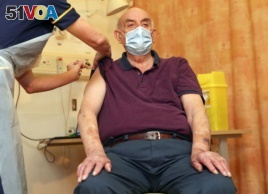
\includegraphics[scale=0.7]{003_voa_20210105.jpg}
\caption{82-year-old Brian Pinker receives the Oxford University-AstraZeneca COVID-19 vaccine from nurse Sam Foster at the Churchill Hospital in Oxford, southwest England on January 4, 2021.}
\end{figure}

By Susan Shand
04 January 2021
The United States says it is considering giving some people half the dose of Moderna's COVID-19 vaccine in order to vaccinate more people.
Moncef Slaoui is the head the country's vaccine program. He said Sunday that officials were discussing the possible plan with Moderna and the Food and Drug Administration (FDA). Moderna's vaccine requires two doses per individual.
He said that giving half of the dose to people between the ages of 18 and 55 will allow the vaccination program to "double the number of people with the doses we have."
He added that just one injection causes an "identical" immunity.
Moderna and the FDA could not immediately be reached for comment.
The U.S. Centers for Disease Control and Prevention said it had injected more than four million people with a first dose of vaccine by Monday morning. It said it had sent out more than 13 million doses.
The U.S. has also approved a two-dose vaccination treatment from drug company Pfizer.
The government's vaccination plan has not been meeting its goals. Officials had hoped to have 20 million people vaccinated by the end of the 2020.
Vaccine race
Britain has administered about one million vaccinations since it approved the Pfizer vaccine in early December. On Monday, it became the first country to use a vaccine developed by Oxford University and AstraZeneca. That vaccine is easier to store and transport.
A new surge of COVID-19 cases is threatening the country's National Health Service. Britain is trying to vaccinate older people and others at higher risk from the disease. Prime Minister Boris Johnson's government has secured 100 million doses of the Oxford/AstraZeneca vaccine.
Eighty-two-year-old Brian Pinker was the first person to get that vaccine outside of experimental use.
Pinker, who has kidney disease, said he was "proud" the medicine was invented in Oxford.
Israel is the world's vaccination leader. More than ten percent of its population is already vaccinated. Israel is now injecting more than 150,000 people a day.
In December 2020, China approved its first COVID-19 vaccine. It is one injection and was created by drugmaker Sinopharm. The government-owned company has said its treatment is 79 percent effective against the virus.
Russia has been providing its COVID-19 vaccine, called Sputnik V, since August. More than 100,000 people have been injected. In November, the government said the treatment was more than 91 percent effective.
New versions
Britain has seen a surge in coronavirus cases in recent weeks as officials struggle to control the spread of a new version of the COVID-19 virus. The new version is far more contagious than others. Officials have recorded more than 50,000 new infections a day since December 29. On Monday, they reported 407 deaths related to the virus. That brings the total number of confirmed COVID deaths in Britain to 75,431.
Britain also reports the presence of a second new version of coronavirus. It appears that version came from South Africa.
Johnson said on Sunday that more restrictions were likely, even with millions already living under the highest level of restrictions.
Starting at midnight tonight, most of mainland Scotland will be in total lockdown, announced Scottish First Minister Nicola Sturgeon.
Europe
In Germany, government spokesman Steffen Seibert said Monday that the government does not regret its decision last year to have the European Union order vaccines for all 27 nations. He said that for a country in the middle of Europe with many borders, "everyone for themselves cannot be the way."
Nearly 265,000 vaccinations have been reported since the program began one week ago. Critics are pointing to faster programs in the U.K., the U.S. and Israel.
Health Ministry spokesman Hanno Kautz said 1.3 million doses of the BioNTech-Pfizer vaccine were delivered to Germany before the end of 2020 and another 670,000 are due on Friday. Germany has 83 million people.
I'm Susan Shand.
The Associated Press and the Reuters News Agency reported this story. Susan Shand adapted it for Learning English. Caty Weaver was the editor.

\begin{messagebox}
Words in This Story
dose – n. the amount of a medicine, drug, or vitamin that is taken at one time
immunity – n. the power to keep yourself from being affected by a disease
surge - n. a move that is very quick and sudden in a particular direction
contagious – adj. able to be passed from one person or animal to another by touching
\end{messagebox}

The United States says it is considering giving some people half the dose of Moderna's COVID-19 vaccine in order to vaccinate more people.
美国称其正考虑给某些人接种一半剂量的新冠肺炎疫苗,以便为更多人接种疫苗。
Moncef Slaoui is the head the country's vaccine program. He said Sunday that officials were discussing the possible plan with Moderna and the Food and Drug Administration (FDA). Moderna's vaccine requires two doses per individual.
蒙塞夫·斯拉维是美国疫苗项目的负责人。他周日表示,有关官员正同莫德纳公司以及美国食品药品管理局讨论这种可能的方案。莫德纳公司的疫苗需要每人注射两针。
He said that giving half of the dose to people between the ages of 18 and 55 will allow the vaccination program to "double the number of people with the doses we have."
他说,给年龄在18到55岁之间的人士注射一半剂量的疫苗,将使疫苗接种计划能够将“现有疫苗的可接种人数翻倍。”
He added that just one injection causes an "identical" immunity.
他还表示,只注射一针剂量会产生“完全相同”的免疫效果。
Moderna and the FDA could not immediately be reached for comment.
莫德纳公司和美国食品药品管理局未能立即发表评论。
The U.S. Centers for Disease Control and Prevention said it had injected more than four million people with a first dose of vaccine by Monday morning. It said it had sent out more than 13 million doses.
美国疾病控制预防中心表示,截至周一早上,已经向超过400万人注射了第一针疫苗。该中心称其已经发放了超过1300万剂疫苗。
The U.S. has also approved a two-dose vaccination treatment from drug company Pfizer.
美国还批准了辉瑞制药公司的一种两剂疫苗疗法。
The government's vaccination plan has not been meeting its goals. Officials had hoped to have 20 million people vaccinated by the end of the 2020.
美国政府的疫苗方案尚未达成其目标。官员们希望在2020年底前接种2000万人。
Vaccine race
疫苗竞赛
Britain has administered about one million vaccinations since it approved the Pfizer vaccine in early December. On Monday, it became the first country to use a vaccine developed by Oxford University and AstraZeneca. That vaccine is easier to store and transport.
英国自12月初批准辉瑞疫苗以来,已经进行了大约100万次接种。英国周一成为采用牛津大学和阿斯利康公司所研发疫苗的首个国家。这种疫苗更易于储存和运输。
A new surge of COVID-19 cases is threatening the country's National Health Service. Britain is trying to vaccinate older people and others at higher risk from the disease. Prime Minister Boris Johnson's government has secured 100 million doses of the Oxford/AstraZeneca vaccine.
新一轮的新冠肺炎病例正在威胁该国的国民医疗服务体系。英国正尝试给老年人和其它高风险人群接种。英国首相鲍里斯·约翰逊领导的政府已经获得了1亿剂牛津大学和阿斯利康公司研发的疫苗。
Eighty-two-year-old Brian Pinker was the first person to get that vaccine outside of experimental use.
82岁的布莱恩·平克是实验用途之外接种该疫苗的第一人。
Pinker, who has kidney disease, said he was "proud" the medicine was invented in Oxford.
患有肾脏疾病的平克表示,他对牛津大学研发的这种药物感到骄傲。
Israel is the world's vaccination leader. More than ten percent of its population is already vaccinated. Israel is now injecting more than 150,000 people a day.
以色列是全球疫苗接种的领跑者。该国10\%以上人口已经接种了疫苗。以色列现在每天给超过15万人注射疫苗。
In December 2020, China approved its first COVID-19 vaccine. It is one injection and was created by drugmaker Sinopharm. The government-owned company has said its treatment is 79 percent effective against the virus.
2020年12月,中国批准了该国第一种新冠肺炎疫苗。它是由国药集团生产的一种注射剂。这家国有企业称其疫苗对新冠病毒的有效率为79\%。
Russia has been providing its COVID-19 vaccine, called Sputnik V, since August. More than 100,000 people have been injected. In November, the government said the treatment was more than 91 percent effective.
俄罗斯自8月份以来一直在接种一种名为Sputnik V的新冠肺炎疫苗。已经有超过10万人接种。俄罗斯政府在11月表示,该疫苗的有效率为91\%以上。
New versions
病毒新变种
Britain has seen a surge in coronavirus cases in recent weeks as officials struggle to control the spread of a new version of the COVID-19 virus. The new version is far more contagious than others. Officials have recorded more than 50,000 new infections a day since December 29. On Monday, they reported 407 deaths related to the virus. That brings the total number of confirmed COVID deaths in Britain to 75,431.
由于官员们难以控制一种新冠病毒变种的传播,英国近几周新冠病毒病例激增。这种新变种比其它类型病毒的感染力更强。自12月29日以来,官方每天录得超过5万例新增感染病例。周一,英国报告了407例与这种病毒有关的死亡病例。这使得英国确诊新冠肺炎死亡总人数达到了75431人。
Britain also reports the presence of a second new version of coronavirus. It appears that version came from South Africa.
英国还报告出现了第二种新冠病毒变种。这种新变种病毒似乎来自于南非。
Johnson said on Sunday that more restrictions were likely, even with millions already living under the highest level of restrictions.
约翰逊周日表示可能会出台更多限制措施,即便已经有数百万人生活在最高级别的限制措施之下。
Starting at midnight tonight, most of mainland Scotland will be in total lockdown, announced Scottish First Minister Nicola Sturgeon.
苏格兰首相尼古拉·斯特金宣布,从今晚午夜开始,苏格兰大部分地区将处于全面封锁状态。
Europe
欧洲
In Germany, government spokesman Steffen Seibert said Monday that the government does not regret its decision last year to have the European Union order vaccines for all 27 nations. He said that for a country in the middle of Europe with many borders, "everyone for themselves cannot be the way."
在德国,政府发言人斯坦芬·塞伯特周一表示,德国政府对去年决定为欧盟所有27个成员国订购疫苗的决定不感后悔。他说,对于一个处于欧洲中部、边界众多的国家来说,“人人只想着自己不是解决办法。”
Nearly 265,000 vaccinations have been reported since the program began one week ago. Critics are pointing to faster programs in the U.K., the U.S. and Israel.
自一周前该计划开始以来,已经报告有近26.5万人接种。批评人士指出英国、美国和以色列推出了更快的疫苗接种计划。
Health Ministry spokesman Hanno Kautz said 1.3 million doses of the BioNTech-Pfizer vaccine were delivered to Germany before the end of 2020 and another 670,000 are due on Friday. Germany has 83 million people.
德国卫生部发言人汉诺·考茨表示,2020年底前已经向德国交付了130万剂由BioNTech和辉瑞公司联合研制的疫苗,周五还将会交付67万剂疫苗。德国有8300万人口。

\subsection{2021年2月19日}
\paragraph{\href{https://www.51voa.com/VOA_Special_English/japan-starts-covid--vaccinations-86319.html}{原文}}

\begin{figure}[H]
\centering
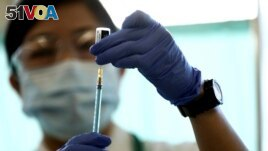
\includegraphics[scale=0.7]{004_voa_20210219.jpg}
\caption{A medical worker fills a syringe with a dose of the Pfizer-BioNTech COVID-19 vaccine at Tokyo Medical Center.(Behrouz Mehri/Pool Photo via AP)}
\end{figure}

By Dan Friedell
17 February 2021
Japan began giving COVID-19 vaccinations to its people on Wednesday. Many other developed countries began vaccination campaigns back in December.
Japan is behind other countries because it asked drug companies to carry out special clinical trials with Japanese people. The country only gave permission for the vaccine on Sunday.
The delay has some people worried that not enough Japanese people will be vaccinated before the proposed start of the delayed 2020 Tokyo Olympic Games.
The Games are now set to begin on July 23, after being delayed by one year because of the coronavirus health crisis.
The first people in Japan to get the vaccine -- made by Pfizer and BioNTech -- are medical workers, old people and people with health problems.
The rest of the Japanese public may be able to get a vaccine in the late spring or early summer.
Japan has a population of 127 million people. At the current rate, not enough people will have the vaccine by the start of the Olympics to make sure everyone is safe.
Officials are struggling to fight opposition among citizens to holding the Games. Recent public opinion studies in Japan found that about 80 percent of those questioned support canceling the Games completely or delaying them again.
But Japanese leaders, including Prime Minister Yoshihide Suga, say they want to move forward with the Games. They say the Olympics will be "proof of human victory against the pandemic."
Japan also wants to show the world it can hold the Olympics before China runs the 2022 Winter Olympics in Beijing. Those Games are set to start in less than one year.
Japan has dealt with the pandemic better than many Western countries. But a recent increase in cases has caused concern. Currently, some parts of Japan are under stronger restrictions than they faced during most of 2020.
Japan is still doing well compared to many other countries. About one person out of every 100,000 is testing positive for the virus. In the United States, that number is almost 25 out of 100,000.
One of the first Japanese people to get the vaccine was Dr. Kazuhiro Araki. He is the president of the Tokyo Medical Center.
He said it did not hurt, adding "I hope we feel more at ease."
Taro Kono is Japan's vaccine minister. He answered criticism about the slow start to the vaccination program by saying it was important to show the Japanese people it would be safe.
"So at the end of the day we might have started slower, but we think it will be more effective," he said.
Japanese leaders say they are working to develop more vaccines in Japan instead of using doses from other countries. More vaccine will arrive next week.
Almost 4 million health care workers are set to be vaccinated in March. Starting in April, the 36 million Japanese people aged 65 and older will be able to receive their shots.
I'm Dan Friedell.
Mari Yamaguchi wrote this story for The Associated Press. Dan Friedell adapted it for Learning English. Ashley Thompson was the editor.

\begin{messagebox}
Words in This Story
clinical trial - n. a test to determine the effectiveness of a new drug or medical technique
pandemic - n. an occurrence in which a disease spreads very quickly and affects a large number of people over a wide area or throughout the world
positive - adj. showing the presence of a particular germ, condition, or substance
dose - n. the amount of a medicine, drug, or vitamin that is taken at one time
\end{messagebox}

Japan began giving COVID-19 vaccinations to its people on Wednesday. Many other developed countries began vaccination campaigns back in December.
日本周三开始给本国民众接种新冠肺炎疫苗。许多发达国家去年12月就开始接种疫苗。
Japan is behind other countries because it asked drug companies to carry out special clinical trials with Japanese people. The country only gave permission for the vaccine on Sunday.
日本落后于其它国家,是因为它要求制药公司对日本人开展特殊的临床试验。该国在本周日才刚刚批准使用这种疫苗。
The delay has some people worried that not enough Japanese people will be vaccinated before the proposed start of the delayed 2020 Tokyo Olympic Games.
这种延误使一些人担心在被推迟的2020年东京奥运会拟开幕前,没有足够多的日本人能够接种疫苗。
The Games are now set to begin on July 23, after being delayed by one year because of the coronavirus health crisis.
这届奥运会由于新冠病毒危机被推迟一年之后,目前定于7月23日开幕。
The first people in Japan to get the vaccine -- made by Pfizer and BioNTech -- are medical workers, old people and people with health problems.
首批接种由辉瑞和BioNTech联合研制疫苗的日本民众包括医务人员、老年人以及存在健康问题的人士。
The rest of the Japanese public may be able to get a vaccine in the late spring or early summer.
其余日本民众也许能够在春末或夏初接种疫苗。
Japan has a population of 127 million people. At the current rate, not enough people will have the vaccine by the start of the Olympics to make sure everyone is safe.
日本有1.27亿人口。按目前的速度,到奥运会开幕时,没有足够多人士接种疫苗以确保每个人都安全。
Officials are struggling to fight opposition among citizens to holding the Games. Recent public opinion studies in Japan found that about 80 percent of those questioned support canceling the Games completely or delaying them again.
有关官员正在努力反驳市民对举办这届奥运会的反对意见。日本最近的民意调查发现,大约80%的被调查者支持完全取消或推迟奥运会。
But Japanese leaders, including Prime Minister Yoshihide Suga, say they want to move forward with the Games. They say the Olympics will be "proof of human victory against the pandemic."
但是包括首相菅义伟在内的日本领导人表示,他们希望继续推进这届奥运会。他们表示,这届奥运会将是“人类战胜大流行的证明。”
Japan also wants to show the world it can hold the Olympics before China runs the 2022 Winter Olympics in Beijing. Those Games are set to start in less than one year.
日本还想向世界展示,它有能力在中国举办2022年冬奥会之前举办本届奥运会。这两届奥运会将在不到1年时间内接连开幕。
Japan has dealt with the pandemic better than many Western countries. But a recent increase in cases has caused concern. Currently, some parts of Japan are under stronger restrictions than they faced during most of 2020.
日本在应对大流行方面要比许多西方国家都做得更好。但是最近的病例激增引发了人们的担忧。目前,日本某些地区受到了比2020年大部分时间都要更严格的限制。
Japan is still doing well compared to many other countries. About one person out of every 100,000 is testing positive for the virus. In the United States, that number is almost 25 out of 100,000.
与其它许多国家相比,日本表现仍然不错。每10万人中大约有1人对病毒呈阳性反应。在美国,这个数字是每10万人接近25人。
One of the first Japanese people to get the vaccine was Dr. Kazuhiro Araki. He is the president of the Tokyo Medical Center.
荒木和宏博士是首批接种该疫苗的日本人之一。他是东京医疗中心的总裁。
He said it did not hurt, adding "I hope we feel more at ease."
他说,接种疫苗不疼,并补充说,我希望大家更加安心。
Taro Kono is Japan's vaccine minister. He answered criticism about the slow start to the vaccination program by saying it was important to show the Japanese people it would be safe.
河野太郎是日本的疫苗大臣。他回应了人们对疫苗接种计划启动缓慢的批评。他说,向日本民众表明接种疫苗的安全,这一点很重要。
"So at the end of the day we might have started slower, but we think it will be more effective," he said.
他说:“所以到头来我们可能会启动缓慢,但是我们认为这样做会更有效。”
Japanese leaders say they are working to develop more vaccines in Japan instead of using doses from other countries. More vaccine will arrive next week.
日本领导人表示,他们正在努力开发更多日本疫苗,而不是使用其它国家的疫苗。下周会有更多疫苗面世。
Almost 4 million health care workers are set to be vaccinated in March. Starting in April, the 36 million Japanese people aged 65 and older will be able to receive their shots.
日本计划在3月份为400万医护人员接种疫苗。从4月开始,3600万名65岁及以上年龄的日本民众将能够接种疫苗。

\subsection{2021年3月1日}
\paragraph{\href{https://www.51voa.com/VOA_Special_English/new-study-black-hole-may-be-larger-than-expected-86383.html}{原文}}

\begin{figure}[H]
\centering
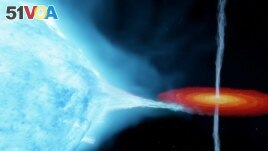
\includegraphics[scale=0.7]{005_voa_20210301.jpg}
\caption{FILE - An artist's impression of the Cygnus X-1 system, with a so-called stellar-mass black hole orbiting a companion star some 7,200 light years from Earth. (International Centre for Radio Astronomy Research/Handout via REUTERS)}
\end{figure}

By John Russell
27 February 2021
A recent study found that the first black hole ever discovered is a lot bigger than scientists first thought.
Black holes are extremely massive space objects whose gravity is so powerful not even light escapes. The black hole, Cygnus X-1, was discovered in 1964. It is well-known for being the object of a friendly bet between two famous scientists.
Researchers found that new observations of Cygnus X-1 showed it is 21 times our sun's mass. That is about 50 percent more massive than scientists had believed.
While it is still one of the closest black holes known, the scientists found it is farther away than earlier estimates suggested. It is 7,200 light years away. A light year is the distance light travels in one year.
Some black holes, like the one at the center of the Milky Way Galaxy, are extremely large. These are called "supermassive" black holes. They can be millions of times more massive than the sun. Smaller black holes are called "stellar-mass" black holes. They have the mass of a single star.
Cygnus X-1 is the Milky Way's largest-known stellar-mass black hole. It is among the strongest X-ray sources seen from Earth, said James Miller-Jones of Curtin University and the International Centre for Radio Astronomy Research in Australia. Miller-Jones led the study that appeared in the publication Science.
Cygnus X-1 turns so quickly that it comes close to the highest rate predicted under physicist Albert Einstein's theory of general relativity, Miller-Jones added.
The black hole brings in material that comes from the surface of the star that it orbits. This star is a "blue supergiant," a very large star about 40 times our sun's mass.
Cygnus X-1 started to exist 4 million to 5 million years ago as a star up to 75 times more massive than the sun. But then it collapsed into a black hole a few tens of thousands of years ago.
The research included data from the Very Long Baseline Array radio telescope. It is made up of 10 observation stations in the United States.
After Cygnus X-1 was first identified as a possible black hole, a friendly bet was made between two physicists, Stephen Hawking and Kip Thorne. Hawking bet against the object being a black hole, while Thorne bet that it was one. Hawking eventually admitted that the evidence suggested Cygnus X-1 was a black hole.
Miller-Jones, the leader of the recent study said, "Indeed, I did not have any wagers riding on these findings."
I'm John Russell.
Will Dunham reported on this story for Reuters. John Russell adapted it for Learning English. Mario Ritter, Jr. was the editor.

\begin{messagebox}
Words in This Story
bet – n. an agreement in which people try to guess what will happen and the person who guesses wrong has to give something (such as money) to the person who guesses right; a wager
source – n. the place where something starts from
wager – n. an agreement in which people try to guess what will happen and the person who guesses wrong has to give something (such as money) to the person who guesses right; a bet
\end{messagebox}

A recent study found that the first black hole ever discovered is a lot bigger than scientists first thought.
一项最新研究发现,人类有史以来发现的第一个黑洞要比科学家最初认为的要大得多。
Black holes are extremely massive space objects whose gravity is so powerful not even light escapes. The black hole, Cygnus X-1, was discovered in 1964. It is well-known for being the object of a friendly bet between two famous scientists.
黑洞是极其巨大的空间物体,其引起是如此之大,甚至连光都无法逃脱。天鹅座X-1黑洞于1964年被发现。它因为成为两位科学家之间友好打赌的对象而闻名。
Researchers found that new observations of Cygnus X-1 showed it is 21 times our sun's mass. That is about 50 percent more massive than scientists had believed.
研究人员发现,对天鹅座X-1的新观测表明其质量是太阳系的21倍。这比科学家之前认为的要大50%。
While it is still one of the closest black holes known, the scientists found it is farther away than earlier estimates suggested. It is 7,200 light years away. A light year is the distance light travels in one year.
尽管它仍然是已知最接近地球的黑洞之一,但是科学家们发现它比之前估计的要远得多。它距离我们有7200光年。1光年是指光在1年当中传播的距离。
Some black holes, like the one at the center of the Milky Way Galaxy, are extremely large. These are called "supermassive" black holes. They can be millions of times more massive than the sun. Smaller black holes are called "stellar-mass" black holes. They have the mass of a single star.
有些黑洞非常大,例如银河系当中的黑洞。这些被称之为“超大质量”黑洞。它们的质量可能是太阳的几百万倍。较小的黑洞被称为恒星级黑洞。它们具有单颗恒星的质量。
Cygnus X-1 is the Milky Way's largest-known stellar-mass black hole. It is among the strongest X-ray sources seen from Earth, said James Miller-Jones of Curtin University and the International Centre for Radio Astronomy Research in Australia. Miller-Jones led the study that appeared in the publication Science.
天鹅座X-1是银河系当中最大的恒星级黑洞。科廷大学和澳大利亚国际射电天文学研究中心的詹姆斯·米勒琼斯说,这是从地球上观测到的最强的X射线源之一。米勒琼斯领导了这项研究,其研究结果发表在《科学》杂志上。
Cygnus X-1 turns so quickly that it comes close to the highest rate predicted under physicist Albert Einstein's theory of general relativity, Miller-Jones added.
米勒琼斯还说,天鹅座X-1的自转是如此之快,以至于接近物理学家爱因斯坦的广义相对论所预测的最高速度。
The black hole brings in material that comes from the surface of the star that it orbits. This star is a "blue supergiant," a very large star about 40 times our sun's mass.
这个黑洞吸取了它所绕行的恒星表面的物质。这颗恒星是蓝巨星, 它是一颗非常巨大的恒星,其质量约为太阳质量的40倍。
Cygnus X-1 started to exist 4 million to 5 million years ago as a star up to 75 times more massive than the sun. But then it collapsed into a black hole a few tens of thousands of years ago.
天鹅座X-1的存在始于400万到500万年前,它是一颗质量是太阳75倍的恒星。但是在几万年前,它坍塌成了一个黑洞。
The research included data from the Very Long Baseline Array radio telescope. It is made up of 10 observation stations in the United States.
这项研究包含的数据来自于甚长基线射电望远镜阵。它是由美国的10个观测站组成的。
After Cygnus X-1 was first identified as a possible black hole, a friendly bet was made between two physicists, Stephen Hawking and Kip Thorne. Hawking bet against the object being a black hole, while Thorne bet that it was one. Hawking eventually admitted that the evidence suggested Cygnus X-1 was a black hole.
在天鹅座X-1最初被认定可能是黑洞之后,斯蒂芬·霍金和基普·索恩这两位物理学家进行了一项友好的打赌。霍金赌这个物体不是黑洞,而索恩赌那就是一个黑洞。霍金最终承认,有证据表明天鹅座X-1是一个黑洞。
Miller-Jones, the leader of the recent study said, "Indeed, I did not have any wagers riding on these findings."
这项最新研究的负责人米勒琼斯表示:“其实我对这些发现没投任何赌注。”

\subsection{2021年4月13日}
\paragraph{\href{https://www.51voa.com/VOA_Special_English/iran-blames-israel-for-nuclear-plant-outage-86655.html}{原文}}

\begin{figure}[H]
\centering
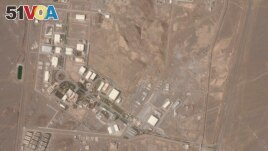
\includegraphics[scale=0.7]{005_voa_20210413.jpg}
\caption{This satellite photo from Planet Labs Inc. shows Iran's Natanz nuclear facility on Wednesday, April 7, 2021. (Planet Labs Inc. via AP)}
\end{figure}
By Bryan Lynn
12 April 2021
Iran has accused Israel of carrying out an attack on a nuclear center that damaged equipment and caused a power outage.
Iranian officials called Sunday's incident at the Natanz nuclear center an act of "nuclear terrorism." They said centrifuges were damaged at the plant. A centrifuge is a device used to increase the purity of uranium for nuclear purposes.
Media organizations reported the Israeli government was behind the action, which was described as a cyberattack. However, Israel did not claim responsibility for an attack or comment directly on the incident.
Speaking to reporters Monday, Israeli Prime Minister Benjamin Netanyahu said Israel would continue efforts aimed at preventing Iran from gaining a nuclear weapon. He said such a device would give Iran the ability "to carry out its genocidal goal of eliminating Israel." He added that Israel "will continue to defend itself against Iran's aggression and terrorism."
A former chief of Iran's paramilitary Revolutionary Guard, General Mohsen Rezaei, said in a message on Twitter that the attack had started a fire.
Iran's Foreign Ministry spokesman Saeed Khatibzadeh said the country's answer to the action should be "to take revenge against Israel." He did not comment further, but added that Israel "will receive its answer through its own path."
Khatibzadeh confirmed that centrifuges at the plant had been damaged. The incident took place one day after Iran announced it had launched new, advanced centrifuge machines at Natanz. Khatibzadeh said only the older centrifuges were damaged.
Iran's improvements in centrifuge technology are designed to permit the country to process uranium faster.
Since January, Iran has begun enriching uranium to as high as 20 percent purity, a technical step away from weapons-grade levels.
The incident came after negotiations began last week in Vienna aiming to bring the United States back into a 2015 nuclear deal with Iran. The deal -- which the U.S. left in 2018 under President Donald Trump -- restricts Iran's nuclear program in exchange for easing U.S. and international sanctions.
The U.S. reestablished economic sanctions after withdrawing from the agreement. Iran answered by violating some of the terms of the deal.
In Vienna, officials from the U.S. and Iran were holding indirect talks. Also taking part were representatives from countries still in the nuclear deal -- Britain, China, France, Germany and Russia.
U.S. Defense Secretary Lloyd Austin arrived Monday in Israel for talks with Netanyahu and other officials. When asked by reporters whether the nuclear discussions might be affected by the incident at the plant Lloyd said, "Those efforts will continue."
In a statement, the White House said it knew about the Natanz attack and that "the U.S. was not involved in any manner."
I'm Bryan Lynn.

\begin{messagebox}
Words in This Story
cyberattack – n. an attempt by attackers to damage or destroy a computer network or system
eliminate – v. remove or get rid of something
revenge – n. the act of doing something to hurt someone because that person did something that hurt you
advanced – adj. having developed or progressed to a late stage
sanction – n. a restriction, usually limiting trade, that are meant to cause a country to obey international law
manner –n. way or method that something is done
\end{messagebox}

Iran has accused Israel of carrying out an attack on a nuclear center that damaged equipment and caused a power outage.
伊朗指责以色列袭击一处核中心,破坏了设备,并造成了停电。
Iranian officials called Sunday's incident at the Natanz nuclear center an act of "nuclear terrorism." They said centrifuges were damaged at the plant. A centrifuge is a device used to increase the purity of uranium for nuclear purposes.
伊朗官员称纳坦兹核中心周日发生的事件是“核恐怖主义”行为。他们表示该工厂有离心机受到了破坏。离心机是一种提高铀纯度用于核用途的设备。

Media organizations reported the Israeli government was behind the action, which was described as a cyberattack. However, Israel did not claim responsibility for an attack or comment directly on the incident.
媒体机构报道称,以色列政府是这场被称为网络攻击的行动的幕后黑手。然而,以色列并未宣称对这起袭击事件负责,也没有直接对该事件发表评论。

Speaking to reporters Monday, Israeli Prime Minister Benjamin Netanyahu said Israel would continue efforts aimed at preventing Iran from gaining a nuclear weapon. He said such a device would give Iran the ability "to carry out its genocidal goal of eliminating Israel." He added that Israel "will continue to defend itself against Iran's aggression and terrorism."
以色列总理内塔尼亚胡周一对记者表示,以色列将继续努力防止伊朗获得核武器。他说,这种武器将使伊朗有能力“实施其消灭以色列的种族主义目标。”他还表示,以色列“将继续抵抗伊朗的侵略和恐怖主义。”

A former chief of Iran's paramilitary Revolutionary Guard, General Mohsen Rezaei, said in a message on Twitter that the attack had started a fire.
伊朗革命卫队前负责人莫森·雷扎伊在推特上发文表示,这次袭击引发了大火。

Iran's Foreign Ministry spokesman Saeed Khatibzadeh said the country's answer to the action should be "to take revenge against Israel." He did not comment further, but added that Israel "will receive its answer through its own path."
伊朗外交部发言人赛义德·哈蒂布扎德表示,作为回应,伊朗将会对以色列展开报复。他没有进一步评论。但是他还表示,以色列将通过自己的途径得到答案。

Khatibzadeh confirmed that centrifuges at the plant had been damaged. The incident took place one day after Iran announced it had launched new, advanced centrifuge machines at Natanz. Khatibzadeh said only the older centrifuges were damaged.
哈蒂布扎德确认该工厂的离心机已被损坏。事件发生前一天,伊朗刚宣布在纳坦兹核中心启动更先进的新型离心机。哈蒂布扎德表示,只有旧型号离心机受到了破坏。

Iran's improvements in centrifuge technology are designed to permit the country to process uranium faster.
伊朗对离心机技术的改进旨在使该国更快地加工铀。

Since January, Iran has begun enriching uranium to as high as 20 percent purity, a technical step away from weapons-grade levels.
自1月以来,伊朗已经开始将铀浓缩至高达20%的纯度,这是接近武器级水平的一项技术步骤。

The incident came after negotiations began last week in Vienna aiming to bring the United States back into a 2015 nuclear deal with Iran. The deal -- which the U.S. left in 2018 under President Donald Trump -- restricts Iran's nuclear program in exchange for easing U.S. and international sanctions.
事件发生前,上周在维也纳开展了旨在使美国重回与伊朗达成的2015年核协议的谈判。这项协议以限制伊朗的核计划换取美国和国际放松制裁,川普总统于2018年带领美国退出了该协议。

The U.S. reestablished economic sanctions after withdrawing from the agreement. Iran answered by violating some of the terms of the deal.
美国在退出协议后重启了经济制裁。伊朗通过违反该协议的某些条款做出了回应。

In Vienna, officials from the U.S. and Iran were holding indirect talks. Also taking part were representatives from countries still in the nuclear deal -- Britain, China, France, Germany and Russia.
在维也纳,来自美国和伊朗的官员进行了间接谈判。仍然留在该协议中的国家的代表也参加了这次会议,这些国家包括英国、中国、法国、德国和俄罗斯。

U.S. Defense Secretary Lloyd Austin arrived Monday in Israel for talks with Netanyahu and other officials. When asked by reporters whether the nuclear discussions might be affected by the incident at the plant Lloyd said, "Those efforts will continue."
美国国防部长劳埃德·奥斯丁周一抵达以色列,与内塔尼亚胡等官员举行了会谈。当记者问到核谈判是否会受到此次事件的影响时,劳埃德表示:“谈判还将继续下去。”

In a statement, the White House said it knew about the Natanz attack and that "the U.S. was not involved in any manner."
白宫在一份声明中表示,它知晓纳坦兹核中心发生的袭击事件,美国没有以任何方式介入。

I'm Bryan Lynn.
我是布莱恩·林恩。






\end{document}


